% File acl2014.tex
%
% Contact: koller@ling.uni-potsdam.de, yusuke@nii.ac.jp
%%
%% Based on the style files for ACL-2013, which were, in turn,
%% Based on the style files for ACL-2012, which were, in turn,
%% based on the style files for ACL-2011, which were, in turn, 
%% based on the style files for ACL-2010, which were, in turn, 
%% based on the style files for ACL-IJCNLP-2009, which were, in turn,
%% based on the style files for EACL-2009 and IJCNLP-2008...

%% Based on the style files for EACL 2006 by 
%%e.agirre@ehu.es or Sergi.Balari@uab.es
%% and that of ACL 08 by Joakim Nivre and Noah Smith

\documentclass[11pt]{article}
\usepackage{acl2014}
\usepackage{times}
\usepackage{url}
\usepackage{latexsym}
\usepackage{graphicx}


% My Package Includes
\usepackage{upquote} % For real apostrophes (see http://tex.stackexchange.com/questions/63345/how-to-make-a-real-apostrophe-or-single-quote-in-latex#63348)
\usepackage{comment}
\usepackage{xcolor}
\definecolor{dark-blue}{rgb}{0.15,0.15,0.7}
\usepackage{hyperref}
%\hypersetup{colorlinks, linkcolor={dark-blue}, citecolor={dark-blue}, urlcolor={dark-blue}}
\hypersetup{colorlinks, linkcolor=black, citecolor=black, urlcolor=black}
\usepackage{booktabs}
\frenchspacing % Normal (single) spaces after periods.  Cf. http://www.read.seas.harvard.edu/~kohler/latex.html
%\usepackage{natbib}
\usepackage[shortcuts]{extdash} % use "\-/" to help LaTeX insert hyphen/pagebreaks
\usepackage[textwidth=0.9in]{todonotes}
\newcommand{\smalltodo}[2][]
    {\todo[caption={#2}, #1]
    {\tiny#2\normalsize}}

% Have \autoref use the special section symbol instead of `section'.
\renewcommand{\sectionautorefname}{\S}
\renewcommand{\subsectionautorefname}{\S}
\renewcommand{\subsubsectionautorefname}{\S}

\newtheorem{requirement}{Requirement}

% GLOSSARIES PACKAGE
\usepackage{glossaries}
\glossarystyle{tree}
\makeglossaries
% commands to run to build the glossaries and acronyms files:
% makeindex -s computel_2014.ist -o computel_2014.gls computel_2014.glo
% makeindex -t computel_2014.alg -s computel_2014.ist -o computel_2014.acr computel_2014.acn

% End My Package Includes

\newacronym{api}{API}{Aplication Programming Interface}
\newacronym{gui}{GUI}{Graphical User Interface}
\newacronym{cl}{CL}{computational linguistics}
\newacronym{nlp}{NLP}{Natural Language Processing}
\newacronym{sil}{SIL}{Summer Institute of Linguistics}
\newacronym{json}{JSON}{JavaScript Object Notation}
\newacronym{npm}{NPM}{Node Package Manager}
\newacronym{bdd}{BDD}{Behavior Driven Development}
\newacronym{scrud}{SCRUD}{search, create, read, update, and delete}
\newacronym{rdbms}{RDBMS}{relational database management system}
\newacronym{igt}{IGT}{interlinear glossed text}
\newacronym{fst}{FST}{finite-state transducer}
\newacronym{cs}{CS}{context-sensitive}
\newacronym{lm}{LM}{language model}
\newacronym{url}{URL}{uniform resource locator}


%\setlength\titlebox{5cm}

% You can expand the titlebox if you need extra space
% to show all the authors. Please do not make the titlebox
% smaller than 5cm (the original size); we will check this
% in the camera-ready version and ask you to change it back.


%\title{LingSync \& the Online Linguistic Database:\\Web Tools for Linguistic Fieldwork}
%\title{LingSync \& the  Online Linguistic Database:\\ New models  for the collection and management of data for Language Communities, Linguists and Language Learners}
\title{LingSync \& the Online Linguistic Database:\\New models for the
    collection and management of data for language communities, linguists and
language learners}

\author{Joel Dunham \\
University of British Columbia,   \\
Department of Linguistics \\
{\tt jrwdunham@gmail.com} \\\And
Gina Cook \\
iLanguage Lab \\
Montr\'eal \\
{\tt gina.c.cook@gmail.com} \\  \\\And
Joshua Horner \\
Amilia  \\
Montr\'eal \\
{\tt ~josh.horner@gmail.com} \\ }

%\author{First Author \\
%  Affiliation / Address line 1 \\
%  Affiliation / Address line 2 \\
%  Affiliation / Address line 3 \\
%  {\tt email@domain} \\\And
%  Second Author \\
%  Affiliation / Address line 1 \\
%  Affiliation / Address line 2 \\
%  Affiliation / Address line 3 \\
%  {\tt email@domain} \\}

\date{}

\begin{document}
\maketitle
%\tableofcontents

\begin{abstract}
LingSync and the Online Linguistic Database (OLD) are new models for the
collection and management of data in endangered language settings. The
Ling\-/Sync and OLD projects seek to close a feedback loop  between field linguists, language communties, software developers and computational linguists  by creating web services and user interfaces which facilitate
collaborative and inclusive language documentation. This paper presents the
architecture of these tools and resources generated thus far (i.e., languages
being documented, numbers and types of entries). We also briefly discuss the
integration of specific computational methods into the systems, including the 
McGill Prosodylab-Aligner which provides automatic audio
alignment of novel data, as well as opportunities of research in semi-unsupervised machine learning of  language
independent morphological analysis, and symbolic language dependent analyzers. 
The paper discusses the requirements of language documentation software, and presents novel data that demonstrates users are aware of existing software, yet continue to actively seek or build alternatives.
\end{abstract}



\section{Introduction}


In this paper we argue that the LingSync/OLD project forms a sustainable new model for data management which can reduce fragmentation in the area of language documentation software 
and facilitate a feedback loop between field workers, language communities, computational linguists and software developers to maximize the results of language documentation efforts for low-resource language communities.
%In this paper we provide an overview of the LingSync/OLD projects as
%well as the resulting data and data uses. 
%To accommodate the diverse audience of computational linguists and language documentation experts of the ComptuEL workshop the paper presents aspects of the project which maybe trivial background for language documentation experts and trivial technical implementations for computational linguists. 
%The LingSync/OLD project was conceived to help
%language communities and fieldworkers collaboratively gather, structure,
%search, and format primary and secondary linguistic data. 
In \autoref{sec:requirements} we argue that
endangered languages fieldwork presents unique challenges and requirements which
are not met by existing software \autoref{sec:existing-software}.  Architectural considerations\footnote{For further discussion of actual user interaction, screenshots and how
LingSync/OLD data can be exported/published in existing online linguistics
repositories such as EOPAS %
\url{http://www.eopas.org/} %
and OLAC %
\url{http://www.language-archives.org/} %
see \cite{lingsync:2012}. For updates on other modules built upon the
LingSync/OLD APIs see the project's completed milestones.%
\url{https://github.com/OpenSourceFieldlinguistics/FieldDB/issues/milestones?state=closed}}
 under LingSync and the OLD which address these requirements are briefly outlined in \autoref{sec:lingsync-old}. 
 The ability of LingSync/OLD to integrate with existing software libraries commonly used in language documentation projects is demonstrated in \autoref{sec:plugins} and finally \autoref{open-data} 
 demonstrates how the LingSync/OLD project is already seeing some closure of the feedback loop both in language learning apps for heritage speakers and in training Kartuli speakers to build speech recognition systems built on LingSync/OLD data. 
 
%While respecting
%community requirements and keeping some data private, teams are able to make
%select data sets accessible and reusable. 

%LingSync%
%\footnote{\url{https://www.lingsync.org/}; Source:
%\url{https://github.com/OpenSourceFieldlinguistics/FieldDB}.} %
%and the Online Linguistic Database (OLD)%
%\footnote{\url{http://www.onlinelinguisticdatabase.org}; Source:
%    \url{https://github.com/OpenSourceFieldlinguistics/old}; Documentation:
%\url{https://online-linguistic-database.readthedocs.org/en/latest/}.} %
%are software tools designed to facilitate linguistic fieldwork, especially that
%which targets endangered languages. The term \textit{linguistic fieldwork} is
%here given broad interpretation; that is, we take it to encompass all efforts
%in the domains of language documentation, description, revitalization, and
%linguistic research whenever these involve the elicitation of primary
%linguistic data from native speakers. The claim that these sub-endeavors of
%linguistic fieldwork are interconnected is central to the argument for the
%utility of LingSync and the OLD. In the endangered languages context, it is
%crucially important to develop tools and methodologies that contribute towards
%reciprocity between these subdomains and their practitioners. This paper argues
%that LingSync and the OLD accomplish this by facilitating data-sharing and
%collaboration among fieldworkers of various stripes and by implementing
%features that contribute to the accomplishment of their various goals.
%
%The argument is structured as follows. In \autoref{sec:fieldwork} we discuss
%the particular challenges of endangered language fieldwork and the
%opportunities for advancing the state of the art. We then argue that LingSync
%(\autoref{sec:lingsync}) and the OLD (\autoref{sec:old}) are beneficial to
%linguistic fieldwork by demonstrating that they facilitate data-sharing and
%collaboration, promote consistency, allow for sophisticated searches, automate
%the creation of segmented audio files and morphological analyses, permit the
%implementation and testing of models of grammatical components, expose
%re-purposable \glspl{api}, and contribute to language learning.%
%\smalltodo{Note: some of these components merit their own sections; for example,
%Learn X, which currently has its own section.}



%%%%%%%%%%%%%%%%%%%%%%%%%%%%%%%%%%%%%%%%%%%%%%%%%%%%%%%%%%%%%%%%%%%%%%%%%%%%%%%%
% Endangered Languages Fieldwork
%%%%%%%%%%%%%%%%%%%%%%%%%%%%%%%%%%%%%%%%%%%%%%%%%%%%%%%%%%%%%%%%%%%%%%%%%%%%%%%%

\section{Endangered languages fieldwork}\label{sec:fieldwork}

Endangered languages are valuable culturally and scientifically, to their
communities of origin \cite{Ironstrack:2012} and to humanity as a whole
\cite{harrison2007languages}. Efforts must be made to document these languages
while there is still time \cite{Good:2012,Thieberger:2012}. The communities from which endangered languages
originate, while also valuing documentation, are equally interested in
increasing the rates at which their languages are transmitted and used
\cite{Myaamia:2001}. In cases where there are no longer any native speakers, a
community may embark upon a language reclamation project that is wholly
dependent upon the the products of past language documentation efforts
\cite{Leonard:2012,Costa:2012}. Alongside such documentation and
revitalization/reclamation projects is research-driven linguistic fieldwork.
These diversely motivated yet interconnected strands within endangered
languages fieldwork conspire to produce a particular set of requirements for
effective software in this domain.

%In the case of the Myaamia project, where there was no access to native speakers, the
%community has lead a reclamation \cite{Leonard:2012} of the language using only
%the products of language documentation efforts from previous centuries
%\cite{Costa:2012}.

%\textit{Joel: I do not quite understand why the Myaamia project's unique situation
%    should be given such prominence here. Note that it's not really even directly
%    related to fieldwork since they have not speakers \ldots This section intro
%    needs more coherence. --Its only because they have been docuenting the process of what it takes for a community to learn a language. they are further along than other projects. if you know others with academic publications you could site those to make it more ballanced.}

%Much scholarly linguistic effort is being directed towards gathering data
%on these understudied languages for the purposes of scientific discovery.

\subsection{Software requirements}
\label{sec:requirements}


\begin{requirement}
	\label{req:primary-data}
       Integration of primary data
\end{requirement}


%\subsubsection{Integration of primary data}
While language communities are demonstrating that it is possible to make use of
only written texts to bring the language into their daily lives as second
language speakers \cite{Ironstrack:2012}, primary audio/video data \emph{in the
form of engaging content} is crucial to fostering native-like proficiency.
%\smalltodo{``creole-like proficiency'' bothers me. Does anyone really strive for
%that? Yes, actually that is waht the Myaamia are striving for. it is why they us the word "reclamation, not revitalization" It also seems inaccurate. Also, it would be nice to have a reference for
%the claim made in the first sentence here. Also, is ``non-inclusive'' better
%than ``un-inclusive''?} %
~Primary audio/video  have formed part of  language documentation efforts since
the time of phonographs, yet only rarely have such audio (or video) products been
made accessible. %We argue in \autoref{sec:requirements} that todate there has been only  insufficient and non-inclusive software
%requirements gathering with stakeholders when existing software were architected.
%  or more likely either exist in archives or have been lost as technologies have changed over time.  
~Securely and efficiently supporting the integration of primary audio/video data
with text artifacts (e.g., dictionaries, grammars, collections of narratives)
is part of the requirements of any modern language documentation effort
\cite{Schroeter:2006} \cite{Good:2012b}.\footnote{For a more detailed discussion of the technical limitations which are no longer blocking the implementation of these requirements see \cite{lingsync:2012}. } 
 

%However, the current state of the art is, in our estimation, conspicuously
%distant from this ideal. Much of the data generated by linguistic fieldwork is
%still stored in handwritten notes or, if digitized, then in documents that are
%oftentimes unstructured, sequestered on local hard drives, or proprietarily
%formatted.

%\subsubsection{Curation of data}


\begin{requirement}
	\label{req:curation}
       Curation of data
\end{requirement}


While most language documentation literature places emphasis on the creation of
artifacts, our experience has shown that a significant percentage of language
documentation hours are actually dedicated to the curation and filtering of the
data in preparation for publication as artifacts.%
\footnote{Such artifacts might include engaging content to be reused in
    revitalization efforts, or citable/traceable data sets used to support
research claims.}
Even ``a funding body like the ELDP cannot get all of its grantees [only 110
out of 216] to deposit in an archive in a timely fashion (or at all)''
\cite{Thieberger:2012}. We argue in \autoref{sec:existing-software} that
facilitating the collaborative curation of data is, in fact, a core requirement
of any data management or content management software, one which is largely
overlooked by existing software (cf.
\autoref{sec:existing-software}).


%In an ideal situation, it would be easy for fieldworkers of various stripes to
%share and reuse the primary data (i.e., transcriptions, translations, and audio
%recordings) as well as primary analytical information (e.g., morphological
%analyses, categorizations, annotations) that are generated by themselves and
%their peers. 
 
 
%\subsubsection{Inclusion of stakeholders}

\begin{requirement}
	\label{req:inclusive}
       Inclusion of stakeholders
\end{requirement}

A sustainable language documentation effort comes from the creation of a
feedback loop where linguistic research benefits language communities,
%\footnote{possibly in the form of language learning/immersion tools for heritage speakers}, 
computational linguistics research on low-resource languages benefits software
libraries, software developers use libraries which do not break content in
low-resource languages,
%\smalltodo{I do not understand the ``non-mainstream languages and writing
%    systems'' qualifier.  Who is using the non-mainstream languages and writing
%    systems? Is that an unsustainable or a sustainable thing? I don't get it. }~
%\footnote{possibly in the form of open source libraries which non-specialized software developers can integrate into their software without needing to understand how it works}, 
~and increased language community presence on the web,  results in more
accessible primary data, which is a benefit to both linguistic and computational
linguistic research.%
%\smalltodo{How can you ``benefit research as primary data''? This sentence needs
%rewriting methinks \ldots}~%
~However, realizing this feedback loop requires, we argue, tools that facilitate
the inclusion of these various stakeholders in the process of language documentation
\emph{while} the project is underway, not \emph{post hoc} when the data is ``polished,''
which in 50\% of projects never happens \cite{Thieberger:2012}. This
inclusivity requirement means that data and data processes must be available in
formats that are usable to both humans---i.e., via \glspl{gui}---and machines---i.e.,
via software libraries and \glspl{api}.
% It is important to point out that there
%must also be support for multiple \gls{gui} integration contexts, minimally one for
%each context where stakeholder populations interact with data and data
%processes, as shown in \autoref{requirements-contexts}.%
%\smalltodo{Why must there be support for all of these ``GUI integration
%    contexts''? Does this mean a GUI for each one of these contexts? --yes The exact
%    meaning of the claim is not clear to me.  Also, it seems like an assertion
%without justification --okay, maybe other readers will feel the same. .}


\begin{table}[h]
\begin{center}
\scriptsize
\begin{tabular}{llll}
      \toprule
      Stakeholders & Default Context & Mobile Context\\\hline\hline
     
      Language Community & Windows &  iPhone, Android\\
      \midrule

	Field Linguists & Mac, Windows, Linux & iPad, Android\\
	  & Praat, Javascript, LaTeX \\
	  \midrule

	Computational Linguists & Linux, Mac, Windows\\
	 & GATE, UIMA, Pip, NLTK\\
	\midrule

	Web Developers & Mac, Linux, Windows\\
	 & Brew, NPM\\

      \bottomrule

\end{tabular}
\caption{Contexts both in terms of operating systems and programming languages/frameworks where data and  data processes must be available.}
\label{requirements-contexts}
 \end{center}
 \normalsize
\end{table}

%, highly searchable and intelligently structured and, where possible, consistent. 

%To secure community trust and engagement the data must have powerful system-wide access control restrictions which work in ways which community members already understand (Facebook, YouTube). "familiar to many Web users" \cite{Farrar:2010}

%In building inclusive tools we will also able to identify these projects which never came to light, as well as the estimate the work hours which are dedicated to the collection of data vs. curation of data.

% \S \autoref{open-data} 

%
%\smalltodo{Elaborate on distinctive needs of endangered languages 
%Say more about how our approach ``relates to the distinctive needs of working
%with endangered languages''
%This touches on the issue of the privacy requirements and whether the scientific
%community should bother with private data. This also relates to the perilous
%nature of much endangered language data. It's very important that research and
%even documentation efforts don't come at the cost of revitalization efforts.}


% Footnotes for SIL tools URLS, not sure if we need them anymore.
%\footnote{\url{http://fieldworks.sil.org/flex/}} %
%\footnote{\url{http://www-01.sil.org/computing/toolbox/}} %
%\footnote{\url{http://www-01.sil.org/computing/shoebox/}} %


%\subsubsection{Openable data }


\begin{requirement}
	\label{req:openable}
       Openable data
\end{requirement}


Endangered languages fieldwork  presents a unique set of
challenges. 
Labs who would like to reuse the data collected by field teams may not be aware of the
post-colonial context in which many fieldwork situations are embedded.
One potential requirement of language communities may be that all or aspects of
the raw data collected by language documentation project be kept confidential for a certain period of time.%
\footnote{Outside of language documentation contexts there are numerous valid reasons for facilitating privacy on data.
As with social websites (Facebook, YouTube), user data is generally considered private and not accessible to data scientists.
Many content curation (Google Docs, WordPress) sites permit private content, or for content to go through a private stage prior to publication.}


In the field it often happens that a speaker will speak quite candidly or
receive a phone call  during a recorded elicitation session and may want to
restrict access to all or parts of that recording for personal reasons.% 
\footnote{Of course, as one reviewer points out, basing claims on private data runs contrary to a core
    tenet of the scientific method, namely that claims must be able to be
    assessed with transparent access to the methods and data used to support
    them.  However in these contexts field linguists generally protect the
    privacy of their language consultants by simply eliciting novel sentences
    which have similar grammatical features for publication, rather than using
the original narrative.} %
In some cases the living speakers of the language are so few that even
anonymizing the data does not conceal the identity of the speaker from other
speakers in the community.
It also happens that particular stories or descriptions of rituals and cultural
practices need to be restricted to just the language community or even to
sub-groups within the community.%
\footnote{It is thus necessary to also empower language communities to produce
their own content for YouTube and other content sites, permitting the community
to manage censorship of  sensitive topics and personal narratives while
creating more public data.}
%In communities where historical knowledge can
%be encoded in oral tradition, it is even possible that the narratives collected
%by fieldworkers might have relevance in a legal context, e.g., in resource
%disputes.


In order to enable access to all team members and stakeholders, including
stakeholders who are distrustful of the project, language documentation
software must support both a non-trivial permissions system but also facilitate
transparency and a social means of pressure which can encourage open
collaboration rather than distrust.  Even language documentation projects using
ad hoc content creation solutions discussed in \autoref{sec:existing-software} cannot be fully inclusive for fear that when
speakers disagree with each other's dialects and they will ``correct"  each
other's data if the social pressure within the system, or the permissions system
doesn't prevent it.  In fact disagreements in data judgements remains an
untapped  indirect source of grammaticality information for linguistics researchers as there are no language documentation
systems which permit inclusion of all stakeholders via traceable user activity, non-trivial permissions systems
and confidentiality of attributes on data. While not all teams will resort to data encryption or privacy, implementing these features introduces transparency and removes barriers of adoption by language communities who are initially distrustful of language documentation projects. 
%In essence, language documentation projects must share requirements with Facebook, YouTube and Google Docs. 


%Language documentation software must enable community involvement even from the most private of language communities, including encryption of sensitive data and the ability for data to change state from closed to open, and open to closed, and individual attributes of data to be closed. 



%The software can also be a means of opening a dialog with the community about ballancing privacy of present speakers and sharing the language with future speakers.


% REVISIT TODO JOEL
\begin{comment}
``To what extent should the scientific community should bother with private data
and to what extent technology for such belongs in scientific conferences.''
This is a good point. I think that the scientific community \textit{should}
bother with LingSync/OLD data. The fact that this reviewer questions this claim
indicates that we have swung too far in the direction of wanting to assure our
users that their data are private. Of course private data is offensive to the
sensibilities of any self-respecting open source programmer and/or academic.
But we also need to recognize and have understanding for the valid requirements
of our users. I think we need to make it clear that there are and will be
public data sets. We need to make it clear that we understand that this is
important too, e.g., for replicability of experiments. We need to build trust
and one way to do that is by using the data that are made public in order to 
generate resources and tools that are valuable to the owners of the data. And 
this is a major goal of the OLD/LingSync (as I see it). These data are rare
and, therefore, valuable. Smart NLP folks can make significant contributions to
language documentation, theoretical linguistic research, language
revitalization, and the better performance of their own models if they tackle
our data.
\end{comment}



%\subsubsection{Users experience}



\begin{requirement}
	\label{req:productivity}
       User productivity
\end{requirement}


Users  are accustomed to using professionally crafted
software built by teams of hundreds of software engineers, software designers and user experience experts
(e.g., Facebook, Gmail, Google Docs, YouTube, Evernote, Dropbox). They can read
their email on all devices, downloading and sync photos and videos
automatically, have offline and mobile data there seamlessly when they need it.
Yet, software built for researchers is often built by computer science students with no experience in software engineering and human computer interaction.
The overwhelmingly  reason users attribute to their use of generic data curation software such as Microsoft Excel or Google Spreadsheets, rather than software specifically designed for language documentation, is due to the productivity of the user experience itself  \cite{lingsync:2012}. 
For many projects the user interface must be customized to maximize productivity during the funded period of the project, in some cases the actual data entry of project can be completed using Google Spreadsheets before an existing language documentation software can be evaluated and/or customized \cite{Troy:2014}. 

%\smalltodo{Ok. But how is this a requirement for language documentation
%    software? Needs spelling out.}



\subsection{Existing software}
\label{sec:existing-software}


% REVISIT TODO JOEL
\begin{comment}
More comparison with other tools
``Compare the systems with other existing tools used by field linguistics
(e.g., Shoebox)''
My dissertation does this a bunch. So does the CCURL submission. So we could
port a bunch of that here. This relates to the specific ``discuss TypeCraft''
injunction from above.
``Some relevant work is cited but other relevant work is missing, notably
TypeCraft''
Ok. This could be as minimal as inserting a reference. However, it may be that
TypeCraft is so revolutionarily splendid that we need to address it in more
detail than that.
\end{comment}


Fieldwork teams typically have the choice between general-purpose content
curation software (Google Spreadsheets, Evernote, Dropbox, MediaWikis,
WordPress etc.), creating/customizing their own tools, or using specialized
field linguistics desktop applications developed by \gls{sil}:  FLEx
\cite{sil-flex}, Toolbox/Shoebox%
\footnote{Toolbox is the community-supported continuation of Shoebox after
    \gls{sil} ceased actively supporting it.} %
\cite{sil-toolbox-info} and/or WeSay\footnote{\url{http://www.sil.org/resources/software\_fonts/wesay}}.
%\cite{WeSay:2007:Online}.

%and insufficient search functionality, %
%\footnote{While FLEx search has advanced significantly over that of
%    Toolbox/Shoebox, with a notably impressive interface for regular expression
%    creation, some highly useful search features are still lacking.} %
%and issues with open access to the source code.%
%\footnote{While both are freely available, FLEx's source is open while
%Toolbox/Shoebox's is closed.} % I really don't want to fault the SIL, they have a huge amount of code on their GitHub!
The SIL tools were developed primarily with practical 
%\smalltodo{I changed ``professional'' back to ``practical''. I am here 
%contrasting ``practical'' with ``theoretical'', cf. the Wikipedia article on
%lexicography. Note also that the reviews of the SIL tools cited here don't
%actually support the claim here. The lexicographical focus claim is my own
%criticism of the SIL tools. Hence my previous formulation \ldots}~%
lexicography in mind, and as such are not ideally suited to research teams. For
research teams, the primary artifacts generated are not dictionary entries but
rather sentences and grammaticality judgments.  Research teams also spend only
a percentage of their hours interacting with data management software
\cite{Butler:2007,rogers10,robinson07}. Unlike professional lexicography teams,
most research teams are unable to impose lengthy training upon all team members.%
%\smalltodo{Sounds odd to ``impose'' training \ldots, sure but we have still not be able to get the PIs of lingsync to complete any training.}

 
%While these tools support many features which are common between lexicographers and field linguists, being written in C\# (a proprietary language owned by Microsoft)  they historically had limited cross-platform support, forcing research teams to either exclude one or more members of the team from the database, or seek ways to share data with team members who could not install the software.%
%\footnote{Neither FLEx nor Toolbox/Shoebox run natively on Mac operating
%    systems. FLEx runs natively on Linux but Toolbox/Shoebox does not.}

Existing language documentation software,  with the exception of WeSay (a
collaborative dictionary tool), have only ad hoc support for collaboration and
inclusive language documentation while the project is active. Toolbox/Shoebox
collaboration is done via a shared network drive or email with no concurrent
editing. FLEx  facilitates collaboration via a Mercurial repository
\cite{FLExSendReceive:2013:Online} which can  support concurrent 
editing in most data entry situations. The benefit of using a full-fledged
version control system is that the history of the data is viewable. 
%\smalltodo{Removed (the to me superfluous) ``with tools familiar to software
%developers and some computational linguists.''}~%
However, as no permissions are built into Mercurial, users with read only
access must use a manual review process to offer their modifications to the
project. In the edge cases which result in more serious merge conflicts, the
team member most experienced in version control systems becomes a
support technician and a bottleneck blocking the rest of the team from data
entry until the conflicts are resolved.  While FLEx does support collaboration,
the support for collaboration requires a small degree of technical
understanding from all team members to avoid merge conflicts.  FLEx
Send/Receive also limits the integration of audio/video primary data, it
% it only
%accepts bmp, jpg, jpeg, gif, png, tif, tiff, ico, wmf, pcx,  cgm, wav, snd, au,
%aif, aifc, aiff, wma, and mp3 formats  \cite{FLExSendReceive:2013:Online} 
 unfortunately does not support formats used by field linguists including .ogg, .avi, .mp4, and .mov and limits the maximum file size to 1MB  \cite{FLExSendReceive:2013:Online}, despite the fact that most elicitation sessions or long utterances can range between 10MB and 200MB. While these may seem like rare edge cases, these edge cases block teams from adopting dedicated language documentation software.
%\smalltodo{Do we have a source backing up this assertion or is this from someone's
%    experience with the system? I think this could be tightened up and/or footnoted:
%no need for a long list of file extensions cluttering the prose, imo.}

%We would argue that it is not in the features lacking in existing field work software, but rather in the non-functional requirements%
%\footnote{Non-functional requirements ``are an overall property of the system as a whole or of a particular aspect and not a specific function. The systems' overall properties commonly mark the difference between whether the development project has succeeded or failed.'' http://en.wikipedia.org/wiki/Non-functional\_requirement}
% of the user experience itself which causes teams to fall back to using .
% 


Over the past decade or so, a number of language-specific collaborative 
websites have arisen, examples of which are  
%Myaamia Project
%\cite{Myaamia:2001}, 
the Yurok Documentation Project \cite{Yurok:2001:Online},
the Washo Project \cite{Washo:2005:Online}, \cite{Cihlar:2008}, the Washo
Mobile Lexicon \cite{WashoMobile:2008:Online}, Karuk Dictionary and Texts
\cite{Karuk:2009:Online} and the Ilaatawaakani project \cite{Troy:2014}.
More recently, collaborative  tools have arisen that, like FLEx and Toolbox,
are not specific to any one language, but unlike FLEx and Toolbox run on all devices in a web
browser.  In this family belong TypeCraft \cite{Beermann:2012}, the OLD
\cite{dunham2014docs}, and LingSync \cite{lingsync:2012}.

TypeCraft uses a MediaWiki UI combined with additional functionality written in
Java for managing collaboration permissions and sharing. TypeCraft falls into
the category of field databases designed by corpus linguists. As such it
imposes upon users closed lists of categories for languages and parts of speech
\cite{Farrar:2010}, which is unacceptable to field linguists who are
dealing with evolving fine-grained analyses of data categories. In addition,
TypeCraft is online only; Farrar correctly points out that the ``limits of cloud computing
are not inconsiderable, especially for fieldworkers who may not have Internet
access'' \cite{Farrar:2010}.%
%\smalltodo{I do not understand what we are trying to convey by the Farrar quote.
%    Are we saying that he wrongly views cloud computing as limited? This needs 
%to be more clear.}

None of the dedicated language documentation software projects surveyed above 
meet the software requirements outlined in \autoref{sec:requirements}. 
We argue this is the reason why so much fragmentation and introduction of novel language documentation tools and software has occurred, with the only stable long term software projects being those which are undertaken by the \gls{sil}.%
\footnote{We would like to point out that the SIL development team is also on GitHub,  a social tool for open source collaboration which will likely yield technical crossover with research teams and more use of HTML5 to facilitate the requirements in \autoref{sec:requirements} in future SIL software. \url{https://github.com/sillsdev}}
%
%\smalltodo{``None of the software are able'' bothers me. Would ``None of the
%    applications'' be inaccurate? If so, then how about ``None of the software
%tools''?}

 %web-based%
%\footnote{We use the term \emph{web-based} to refer to tools which run online
%or offline in a browser and/or mobile device via the use of native interfaces
%and web services, as opposed to traditional offline desktop applications where
%there is little to no server side component.} %


%EOPAS is for publishing ELAN or Toolbox, not for editing... im pretty sure.
% EOPAS.%
%\footnote{\url{http://www.eopas.org/}} %


%In order to appreciate the significance of web-based collaborative fieldwork
%software, it may be necessary to expand one's preconceptions of what linguistic
%fieldwork looks like in practice. 
%Clearly there is an enduring appeal
%to the vision of the intrepid field linguist on a weeks-long journey to a
%remote and conspicuously Internet-less location in Papua New Guinea or Amazonia
%labouring at collecting texts from which to extract a descriptive phonology,
%morphology, and lexicon of some all-but-undiscovered language. 
%However, this
%romantic vision is now arguably something of an anachronism, and certainly it
%is not the full picture. 
%Present-day endangered languages fieldwork, especially
%in North America, is often conducted in universities, urban centers, or on
%reservations in speakers' houses with wireless access and by groups of
%researchers who are already well versed in the descriptive grammars and are
%working to elicit the syntactic, semantic, and pragmatic knowledge that depends
%upon these lower-level insights. 
%As linguists with experience in this type of
%fieldwork-based research, the developers of LingSync and the OLD can attest to
%the fact that collaborative web-based tools for data storage and analysis respond
%to a very real requirement. 
%In these contexts, great strides can be made simply
%by having easy, web-based, and highly searchable access to one's previously
%elicited data and that of one's peers and predecessors.



\section{New models for data collection and management}

\label{sec:lingsync-old}

\subsection{LingSync}\label{sec:lingsync}

LingSync is an open source project which began on April 20th 2012. 
LingSync is composed of existing and novel open source software modules (rich client-side web
components and task specific web services) which allows all stakeholders of a
language documentation effort to collaboratively create corpora of primary
analyzed and unanalyzed language data \cite{lingsync:2012}.

To meet Requirement \autoref{req:productivity},
LingSync uses a quasi-blackboard system architecture similar to
Android,\footnote{\url{http://developer.android.com}} where modules can be
registered to perform certain tasks, and users can discover and choose between
registered modules. Similar to Praat,\footnote{\url{http://praat.org}}%
%\smalltodo{Is the Praat comparison really contributing anything here? Also, I
%    do not really understand what an ``audit trail'' is or what it means to
%``generate a script by clicking''. This is unclear, to me at least.}~%
all events in the system provide an audit trail which can be used by users,%
\footnote{In the case of Praat users are able to generate automation scripts by clicking to create a repeatable sequence of events.}
but also serve as data for automated reasoning
engines, should labs choose to use the make use of the audit data to assist in data cleaning 
(Requirement \autoref{req:productivity}) and data quality (Requirement \autoref{req:openable}).

Based on the LingSync team's collective prior experience as field linguists, research
assistants, professional lexicographers, and linguists in the language
technologies industry, we hypothesized that perhaps 50\% of data
curation/cleaning tasks are monotonous, repetitive and consistent and thus are
candidates for data manipulation which is best done by machines or
crowdsourcing rather than by one individual human for extended periods of time.
However, we lacked the data to accurately quantify this hypothesis. 
The automation of tasks in field linguistic research is rarely done, and
for good reason. Unlike corpus linguistics, field linguistics seeks
fine-grained analysis of novel data on undocumented languages which means that
data curators must be sensitive to the slightest ``off'' feeling of analysis
which could easily be flattened by over-generalizing cleaning scripts. 
Automated modifications must be fully traceable in their motivations so as to
detect side effects of cleaning long after the cleaning has happened. They must
also be easily undoable so as not to introduce consistency or systematicity in
the data which is not there. %
%\smalltodo{``automatically undoable'' sounds wrong to me. We don't want the system
%to automatically undo its automatic modifications, right? We want to be able to
%easily undo the system's automatic modifications.}~
To better identify the role of machines in data
cleaning in a language documentation context, LingSync's implementation
collects the data required to more accurately identify the ratio tasks best done by machine to tasks best done by humans. 
%of machine
%consistency vs. human reasoning tasks.%
%\smalltodo{I do not understand this last sentence. This is a ratio of what to what?}

The potential time saving features of LingSync's system design will not bear
usable data without the explicit and overarching goal of providing a user
friendly experience for both expert and novice users with differing data description vocabularies and interests \cite{Troy:2014}.  Notable user facing
features include complete user interface customization, powerful searches over the data sets, encryption at a field
level, flexible enforcement of data consistency, social collaborative software
features, an inclusive permissions system, pluggable statistical machine
learning algorithms for building semi-automatic glossers, numerous task
oriented web services which wrap existing libraries and scripts for audio,
video, image and text analysis, two native Android \glspl{gui} which function
offline (Learn X and the Elicitation Session Recorder) and five browser-based
\glspl{gui} (the Prototype, Spreadsheet,  Activity Feeds, Corpus Pages, 
Lexicon Browser), one of which functions offline and provides flexible import
and export functionality.  For up-to-date examples of \gls{gui} interaction
readers are encouraged to search for LingSync on YouTube, as of April 2014
there are over 40 videos made by users demonstrating diverse features in the
systems.


\begin{comment}
\smalltodo{Clearly identify intellectual contribution
``Clearly identify [our] intellectual contribution, and how it addresses the
inadequacies of the state of the art''
This is a pretty general criticism, but it speaks to the lack of coherence in
the paper. This could be addressed by fixing the introduction and better
structuring the paper.
The state of the art is lacking. We need more data-sharing. We need to marshal
CL/NLP and software engineering advances towards endangered language fieldwork
(s.l.) efforts.  We need programming-as-fieldwork to be recognized. We need to
facilitate data reuse so that fieldwork is more efficient, faster. We need to
make it easier for academics to give back to language communities while still
fulfilling their grant obligations. LingSync/OLD does this.}
\end{comment}



\begin{comment}
\smalltodo{Bolster facilitation of collaborative fieldwork claim
``Most the evidence for this (i.e., LingSync/OLD's facilitation of
collaboration) in the paper concerns `collaboration to produce code for
making tools' not `collaboration to do the actual documentation'{}''
I am not quite sure why this reviewer interpreted the paper in this way.
I guess we need to emphasize \textit{how} LingSync/OLD facilitate linguistic
fieldwork, and further support the argument for this claim. Also, the
abstract seems to emphasize the ``develop these tools collaboratively''
idea more than the ``use these tools to do collaborative fieldwork better.''}
\end{comment}


LingSync's libraries and components are built entirely using HTML5 technologies
using current best practices for rich JavaScript client-side apps including
\gls{bdd} testing, and build and dependency management frameworks analogous to
Java's Junit, Gradle and Maven.\footnote{As of 2014 these are Jasmine (testing), Grunt (build automation), and \gls{npm} (dependency management)\\
\url{http://jasmine.github.io}, \\
\url{http://gruntjs.com} \\
\url{https://npmjs.org}}
%run on the Node.js%
%\footnote{\url{http://nodejs.org/}} %
%software platform. 
Data is stored in \gls{json} using Apache CouchDB%
\footnote{\url{http://couchdb.apache.org/}} %
on the server-side (permitting scalable, decentralized, and fully replicated data
stores) and IndexedDB on the client-side. Nearly all logic is performed on the
client-side which permits the users to go offline and consume low bandwidth
when there is limited connectivity.
%, with the LingSync
%Prototype using the Backbone%
%\footnote{\url{http://backbonejs.org/}} %
%framework and LingSync Spreadsheet the Angular%
%\footnote{\url{http://angularjs.org/}} %
%framework.


\begin{comment}
\smalltodo{Overemphasis of web-based-ness
``The dichotomy between web-based (in their terminology) and non web-based
technology seems to be overemphasized. In many field situations web access is
not available, and the distinction is then reduced to whether one decides
to upload data to a repository or not, whenever there is web access.''
I do not agree. I think that the reviewer sees it this way because we have not
presented the argument well enough. The point is that collaboration and
data-sharing will help to advance linguistic fieldwork in all of its aspects. 
You don't just upload your work to a repository for the benefit of others (at
least that's not the way I envision the OLD). You do preparatory research by
searching a LingSync corpus/ OLD app in order to discover which of your
questions can be answered in this way. This gives you a headstart. Then you do
fieldwork and have a better chance of eliciting novel and interesting data. 
Then you contribute back to the system, hopefully in a manner that is
internally consistent or, better yet, consistent with the conventions of your
peers. Then your data give your peers a headstart.}
\end{comment}


%
%The LingSync Prototype%
%\footnote{\url{https://chrome.google.com/webstore/detail/lingsync-prototype/eeipnabdeimobhlkfaiohienhibfcfpa}} %
%is a single-page client-side web application (SPA) that can run offline as a Chrome App (using IndexedDB for persistence) and can
%sync data with the server-side (CouchDB) storage when connectivity is restored.
%This online/offline functionality combines the best of both worlds: the
%cross-platform, collaboration, and data-sharing potential of a web application
%with the offline functioning of a desktop application. In addition, the
%LingSync Prototype provides an interface for customizing the \emph{datum}
%schema, a flexible import feature that helps users to upload data with a wide
%range of structures, export to .zip, .csv, .tex, .txt, .json, .xml, peer to
%peer full replication, and an interface for performing complex searches.
%
%LingSync Spreadsheet%
%\footnote{\url{http://app.lingsync.org}} %
%is a single-page client-side web application with an interface that
%focuses solely on data entry. LingSync Spreadsheet was designed to appear
%spreadsheet-like so as to provide maximum productivity for students in field
%methods courses with no need for additional training, but with the added
%benefit of morpheme segmentation and gloss suggestions.

\subsection{OLD}\label{sec:old}

The OLD also exposes RESTful web services for \gls{scrud} operations. 
A language-specific OLD web service allows for concurrent
multi-user read/write access to a relational fieldwork database. 

%This section
% reviews the database schema, the graphical user and
%application programming interfaces, the search and morphological parsing
%functionalities, the implementation technologies, and the data present on
%currently deployed OLD applications.



The OLD is written in Python using the Pylons web framework%
\footnote{\url{http://www.pylonsproject.org/projects/pylons-framework/about}} %
and an SQLAlchemy-mediated interface to the \gls{rdbms}%
\footnote{Both MySQL and SQLite are supported.} %
It exposes a RESTful \gls{api} where the content in the body of HTTP 
requests and responses is formatted as \gls{json} throughout.%
%\footnote{File data can be Base64 encoded and passed as values of JSON objects.
%However, such encoding is costly and is therefore optional.} %
%The \gls{gui} of the OLD v. 0.2 is dynamically generated HTML, CSS, and JavaScript (YUI \& jQuery).



The \gls{gui} of the OLD is a collection of dynamically generated HTML pages
containing a) web forms for creating and updating OLD objects and b)
representations of text and \emph{form} objects (in \gls{igt} format) with
embedded representations of associated files. OLD texts, search results, and
individual \emph{forms} can be exported in (Xe)LaTeX, TSV, and plain text
formats.

A notable feature of the OLD \gls{gui} is its provision of visual feedback on the
extent to which user-generated morphological analyses match existing lexical
entries in the database. That is, when a user creates a morphologically complex
\emph{form}, the IGT representation indicates, via color-coded internal links,
whether the morpheme shapes and glosses match current lexical entries. This
feature has proved to be quite useful in helping groups of fieldworkers to
generate consistent morphological analyses.



\subsection{LingSync/OLD}

While LingSync and the OLD arose independently and consequently use different
technology stacks, the teams behind the tools have largely complementary interests and are collaborating on
future developments in order to combine strengths and reduce fragmentation of
efforts. In the coming two year partnership we expect to bring OLD's glossing user interfaces, 
logic for connecting documents to utterances as well as structural search and morphological 
parsing into the LingSync plugin architecture, with OLD user interfaces being used by field 
linguists and LingSync user interfaces being used by language community members and 
computational linguists. When referring collectively to both tools, we will henceforth use the
term LingSync/OLD.


%\section{LingSync/OLD's contribution}
%
%
%%The core virtue of LingSync/OLD, is that they facilitate social collection and curation by language documentation teams of web-accessible stores of primary language data.
%%% that
%%%would otherwise remain sequestered on local hard drives and handwritten notes,
%%%and thus largely inaccessible. 
%%This is especially important in the context of
%%endangered languages where numbers of fluent speaker are rapidly declining
%%\cite{fphlcc10}. Beyond existing tools, LingSync/OLD also
%%provide RESTful JSON-mediated APIs which enable labs who are already
%%collaborating with computational linguistics/software engineering labs to
%%customize their own data automation pipelines by incorporating their own
%%in-house tools.
%%
%%
%%Given the post-colonial context of many fieldwork situations, there
%%is an entirely understandable distrust of the dominant society that may result
%%in speakers or communities adopting a generally cautious (or even zero
%%tolerance) approach when it comes to sharing language data via a web-based
%%application. LingSync/OLD do, in fact, comply with this
%%requirement by requiring authentication prior to data access, keeping data
%%private by default, and, in the case of LingSync, allowing contributors to
%%encrypt their data. Data is to be made public through LingSync/OLD only after
%%an intentional decision to do so and in accordance with speaker and community
%%requirements, which teams are encouraged to document in their corpora's Terms of
%%Use, Copyright and License information.
%
%
%In this paper we hope to demonstrate that the  LingSync/OLD project is a plugin architecture conceived, researched and implemented by field workers for language documentation teams, and is a successful implementation of the requirements outlined in \autoref{sec:requirements}.
%%a vehicle of cross pollenation and interdisciplinary inclusion among the diverse stakeholders of a language documentation effort, including but not limited to field linguists, language community members, software developers and computational linguists.
%%; there is a real need for research software to be built using software engineering  industry best practices which can expedite the 
%%accomplishment of fieldwork on endangered languages.
%
%\begin{enumerate}
%    \item Inclusion of stakeholders
%%    ---i.e., linguistic researchers,
%%        descriptive linguists, pure documentarians, revitalizers, and
%%        educators---can work in a way that is mutually beneficial.
%%        The software lowers barriers to re-purposing of data.
%%    \item programming-fieldlinguists
%%    , not by third parties introduces a novel holistic way of thinking about language documentation software.  LingSync/OLD don't have
%%        to blow FLEx/Toolbox/TypeCraft/EOPAS/etc. out of the water to be valuable.
%    \item Openable data
%%     --- this does not mean
%%        that all LingSync/OLD data are private or that computational linguists
%%        should avoid this domain. To the contrary, computational linguistics has
%%        a lot to offer here; lots of low-hanging fruit, as they like to say.
%\item Indirect data which might not have otherwise been envisioned % I want to say something here to the effect that we are excited by
%%        the implications of this claim, namely that 
%%        software engineers and
%%        computational linguists will see in LingSync and the OLD opportunities
%%        to contribute to aspects of linguistics and linguistic fieldwork that
%%        they might not have otherwise envisioned
%\end{enumerate}





\section{User adoption}

\begin{comment}
\smalltodo{
``I would like to know the opinions of field linguists about the systems''
Well, we are field linguists ourselves. I know the lingsync team has collected some of this.
So have I for the OLD. There is definitely more we could say here \ldots At the
very least, we could make it clear that these systems were developed by field
linguists for field linguists. I, at least, have no formal training in software
engineering and little formal training in NLP \ldots But yeah, dig up those user
comments \ldots maybe. ``Thanks for making a really nice tool.'' Rikker
``Keep up the great work on LingSync''  Anna}
\end{comment}


In the past 1.5 years since LingSync was launched over 300  unique
users  have registered for LingSync, despite the availability of a sample user (username: LingLlama, password: phoneme). We argue this demonstrates there is a general interest in a novel, even  unheard of, language documentation software, despite the largely reccommended  solutions discussed in \autoref{sec:existing-software}.
% reached a level that is perhaps surprising given its limited target
%audience of field linguistics teams. 
\autoref{lingsync-data} provides an
overview of the corpora being edited using the system. Currently there are
about 13,400 active records, 38 active users, 15 active corpora, and 1GB of
primary audio/image/text data. There are currently no published measures of user attrition in language documentation projects, however social websites/mobile apps reportedly a  30\% retention rate is not a cause for concern\footnote{There are no official published statistics but developers on StackOverflow report averages to be 30\%. http://stackoverflow.com/questions/6969191/what-is-a-good-active-installs-rate-for-a-free-android-app} we expect that the low ratio of active vs registered users (12\%) is due to both the multi task nature of language documentation projects and early launch of LingSync while it was still in the alpha testing and the requirements gathering phase. We will know more as the retention rate changes over time and in correlation to the release of new modules.
%\smalltodo{I changed the wording of the initial sentence here. I hope that's ok.
%I also removed ``LingSync.org''.}
%For privacy reasons, we do not know which languages are represented
%in the system. 


\begin{table}[h]
\begin{center}
\scriptsize
\begin{tabular}{lrrrr}
      \toprule
                     ~ &  Active & Investigating & In-active & Total\\
      \midrule
      Public Corpora  &       2 &   1 &   2 & 5 \\ 
      Private Corpora &      15 &  37 & 321 & 373\\ 
      Users           &      38 &  43 & 220 & 301 \\
      Documents & 13,408 & 2,763 & 4,541 &23,487\\
      Disk Size & 1GB & .9GB & 5.3GB& 7.2GB\\
      
      \bottomrule

\end{tabular}
\caption{Data in LingSync corpora (Feb 14, 2014).
Active corpora: $>$300 activities; Investigating corpora: 300-10 activities; Active users: $>$100 activities; Investigating users: 100-10 activities.}
\label{lingsync-data}
 \end{center}
 \normalsize
\end{table}



%\subsection{Extant OLD Data}

There are currently nine language-specific OLD applications in use. In total,
there are about 19,000  records (primarily sentences), 300 texts, and 20 GB worth
of audio files.  There are 180 registered users across all applications, of
which 98 have entered and 87 have elicited at least one record. The applications
for Blackfoot, Nata, Gitksan, Okanagan, and Tlingit are seeing the most use. The
exact figures are summarized in \autoref{old-data}.\footnote{
Note that the values in the speakers column are taken from Ethnologue 
\url{http://www.ethnologue.com}  
and are provided only to give a rough indication of the speaker populations of
the languages. Also, the three-character codes in the first column are the ISO
639-3 
\url{http://www-01.sil.org/iso639-3} 
identifiers of the languages.}


\begin{table}[h]
 \begin{center}
     \scriptsize
\begin{tabular}{lrrrrr}

      \toprule
      language &                     \emph{forms}  & texts & audio & GB   & speakers \\
      \midrule
      Blackfoot (\textit{bla}) &     8,847  & 171   & 2,057 & 3.8  & 3,350    \\ % 11,075 4047074461 bytes
      Nata (\textit{ntk}) &          3,219  & 32    & 0     & 0    & 36,000   \\ % 3,251  0 bytes
      Gitksan (\textit{git}) &       2,174  & 6     & 36    & 3.5  & 930      \\ % 2,216  3787227136 bytes
      Okanagan (\textit{oka}) &      1,798  & 39    & 87    & 0.3  & 770      \\ % 1,924  349478912 bytes
      Tlingit (\textit{tli}) &       1,521  & 32    & 107   & 12   & 630      \\ % 1,660  12906459136 bytes
      Plains Cree (\textit{crk}) &   686    & 10    & 0     & 0    & 260      \\ % 696    0 bytes
      Ktunaxa (\textit{kut}) &       467    & 33    & 112   & 0.2  & 106      \\ % 612    176128000 bytes
      Coeur d'Alene (\textit{crd}) & 377    & 0     & 199   & 0.0  & 2        \\ % 576    28659712 bytes
      Kwak'wala (\textit{kwk}) &     98     & 1     & 1     & 0.0  & 585      \\ % 100    7450624 bytes
      TOTAL &                        19,187 & 324   & 2,599 & 19.8 &         \\ % 22,110 21302477981 bytes
      \bottomrule

\end{tabular}
\caption{Data in OLD applications (Feb 14, 2014)}
\label{old-data}
 \end{center}
 \normalsize
\end{table}



%\section{Data Structure}
%
%\subsection{LingSync}
%
%A LingSync database is referred to as a \emph{corpus} and contains
%\textit{datum}. The creator of a corpus controls access to that corpus and can
%grant read-only, read/comment, read/write, write-only and administrator access
%to other registered users. A \emph{datum} is a general-purpose linguistic
%unit---generally, a word, sentence or story---whose attributes are
%customizable. However, due to defaults in the LingSync data entry \glspl{gui}, each
%datum tends to have values for the following attributes: utterance (i.e., an
%orthographic, phonetic, or phonemic transcription), morphemes (i.e., segmented
%morpheme forms), glosses, translation, in addition to tags, comments, and a set
%of associated audio, image or video files. 
%
%\begin{figure}[h]
%\scriptsize
%\begin{verbatim}
%{
%       "label": "utterance",
%       "value": "Kichanaywan punqota",
%       "mask": "xxxxxxxxxxxx xxxxxxx",
%       "encrypted": "",
%       "shouldBeEncrypted": "true",
%       "help": "Unparsed utterance in the language, in 
%          orthography or transcription. Line 1 in your 
%          LaTeXed examples for handouts.",
%       "showToUserTypes": "all|machine|linguist",
%       "userchooseable": "disabled"
%}
%\end{verbatim}
%
%\caption{LingSync datum are composed of any number of DatumFields, with
%minimally the attributes above.}
%\label{lingsync-datastructure}
%\end{figure}
%
%LingSync uses new technology for building scalable decentralized data stores,
%specifically storing the data in a NoSQL, document database (Apache CouchDB%
%\footnote{\url{https://couchdb.apache.org/}}%
%) and therefore providing a non-rigid schema that allows for customization,
%adaptation, extension and inclusion of contributors' existing data structures.
%The use of a document store (similar to Toolbox) rather than a relational
%database allows data schema to change, which enables researchers to customize
%and modify data entry fields at any point during the course of research. Each
%\emph{datum} is traceable to a source (be it a publication or an elicitation
%session). The \glspl{gui} for interacting with the LingSync corpus module allow for
%bookmarking data into ordered lists labeled \textit{data lists} which can be
%used for publishing data sets or tracking data which must be cleaned or
%verified.
%
%LingSync takes special precautions to ensure privacy of data. All data is
%private by default, i.e., can only be accessed by authenticated users who have
%authorization for the corpus in question. Data can be encrypted at the
%attribute level, providing more fine-grained control over data access while
%permitting the corpus to be opened and with confidential items ``blacked'' out.
%A contributor may choose to publicize subsets of their data while keeping
%others encrypted and private, in accordance with the requirements of the
%speakers and communities who provide the data.
%
%
%
%\subsection{OLD}
%
%A simplified UML%
%\footnote{\textit{UML} (Unified Modeling Language) is a standard for creating
%    a visual representation of the design of a system. In \autoref{old-uml}, the
%    boxes represent tables in a relational database, and the lines and their
%    labels the relations between the tables. Thus a form has zero or one
%    categories while a category has zero or more forms; a form has one or more
%translations and a translation has exactly one form; etc.} %
%representation of the OLD schema is provided in
%\autoref{old-uml}. 
%
%\begin{figure}[h]
%\begin{center}
%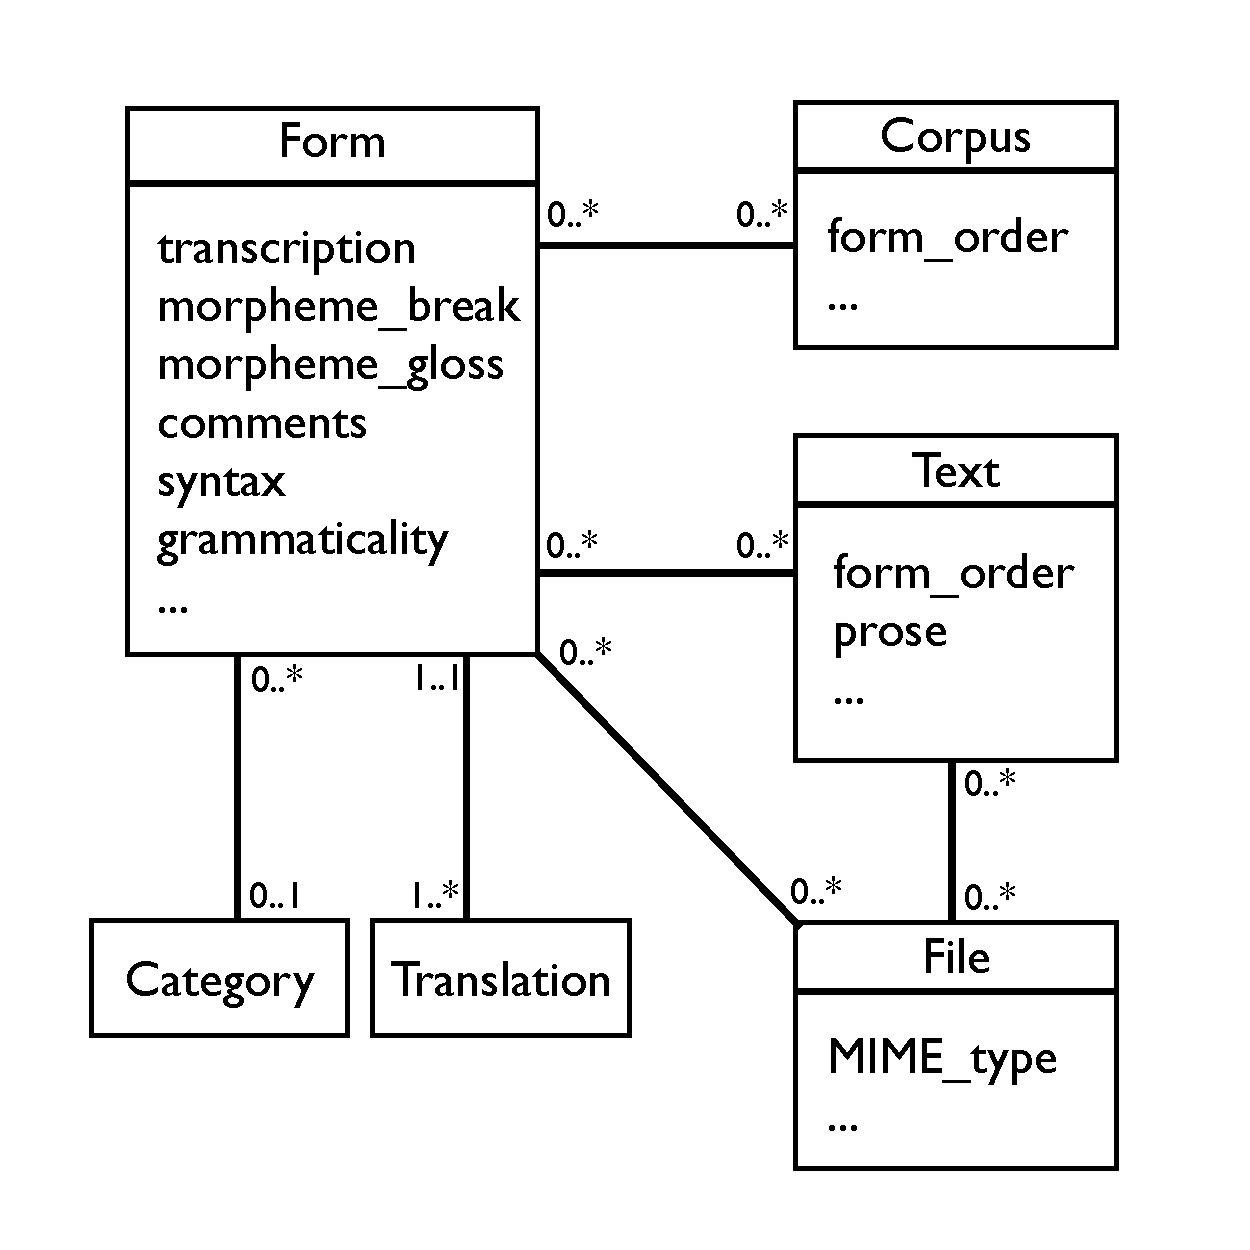
\includegraphics[scale=0.35]{images/OLD_relational_model_UML.pdf}
%\caption{UML diagram of the OLD's relational model (abbreviated).}
%\label{old-uml}
%\end{center}
%\end{figure}
%
%The core object/resource of an OLD web service is the \textit{form}, which is
%used to represent morphemes, words, phrases, or sentences. A \emph{form} has
%attributes for (orthographic and phonetic) transcriptions, a morphological
%analysis (i.e., morpheme segmentation, glosses, and categories), a syntactic
%representation (e.g., a phrase structure tree in bracket notation), metadata
%(e.g., provenance), and related media files (e.g., audio/video recordings).
%Ordered pointers to OLD \emph{forms} are used to create both formatted texts
%(exportable as LaTeX) as well as corpora, including treebanks that can be
%searched structurally via an interface to the TGrep2%
%\footnote{\url{http://tedlab.mit.edu/~dr/Tgrep2/}} %
%utility. The model can also store morphological parser objects and their
%sub-components, i.e., finite-state transducer implementations of phonological
%and morphotactic models (cf. \cite{beesley2003finite}) and $N$-gram language
%model-based (cf.  \cite{manning1999foundations}) implementations of parse
%disambiguators.






\section{Reusing existing tools and libraries}
\label{sec:plugins}

%\smalltodo{Demonstrate utility of our approach
%``Demonstrate the utility of our approach, don't merely assert it!''
%This overlaps with some of the other criticisms. I think we address it by more
%clearly arguing why LingSync/OLD is good, i.e., motivating the need for
%data-sharing, collaboration, effective search, automated morphological
%analysis, model implementation for research, automated generation of audio file
%clips, facilitating the creation of consistent data sets, etc.}

Both the LingSync and the OLD projects were founded with the goal of making it easier to integrate existing language documentation tools and software libraries popular among feild linguists to better automate data curation (Requirement \autoref{req:curation}) and improve data quality (Requirement \autoref{req:openable}). There have been numerous plugins in both systems to this end, however in this paper we will discuss only those which may be of most interest to computational linguists working on low-resource languages: morphological parsers in \autoref{sec:farley},  \autoref{sec:old-parsers} and  \autoref{sec:lingsync-glosser} which are a precursor for Information Retrieval and Machine Translation tasks, and  phone level alignment of audio and text in  \autoref{sec:aligner} which is a precursor for acoustic model training in Speech Recognition systems.




\subsection{Existing Morphological Parsers}
\label{sec:farley}

\autoref{lingsync-parse} illustrates the use of the Inuktitut parsing web service which wraps an existing
morphological analyzer for Inuktitut built in Java \cite{Farley:2012:Online}.


\begin{figure}[h]
\scriptsize
\begin{verbatim}
$ curl --cookie my-cookies.txt\
  --request GET\
  https://api.lingsync.org/v2/elanguage/iu/
  parses/arraagunullu
\end{verbatim}
\normalsize
\caption{Inuktitut morphological analyzer request.}
\label{lingsync-parse}
\end{figure}




\subsection{Novel Morphological Parsers}
\label{sec:old-parsers}


An OLD web service provides functionality that allows users to create any
number of morphological parsers. The phonological mappings of these parsers
are declared explicitly, using a formalism---\gls{cs} phonological rewrite
rules \cite{chomsky68}---that is well understood by linguists. The lexicon,
morphotactic rules, and parse candidate disambiguator components are
automatically induced from corpora specified by the user. The fact that this
implementation requires a good deal of explicit specification by the user
should not be considered a demerit. By granting linguist fieldworkers a good
degree of control over the specification of phonological, lexical, and
morphotactic generalizations, the parser functionality allows for the automatic
testing of these generalizations against large data sets. This assists
in the discovery of counterexamples to generalizations, thereby expediting
the improvement of models and advancing linguistic research. The OLD
morphological parser implementation can, of course, co-exist with and
complement less expert-dependent machine learning approaches to creating
morphological parsers.

The core component of an OLD morphological parser is a morphophonology that is
modelled as a \gls{fst}%
\footnote{\glspl{fst} are constructed using the open source finite-state
compiler and C library foma: \url{http://code.google.com/p/foma}} %
and which analyzes transcriptions to morphological analyses, i.e., morpheme
segmentations, glosses, and categories. The morphophonology \gls{fst} is the
composition of a phonology \gls{fst} that is created explicitly by the user
(using \gls{cs} phonological rewrite rules) and a morphology (i.e., lexicon and
morphotactic rules) that is induced from corpora constructed by the user, cf. 
\cite{beesley2003finite,hulden2012}. When the morphophonology returns multiple
parse candidates, the system employs an $N$-gram \gls{lm}%
\footnote{OLD $N$-gram \glspl{lm} are estimated using MITLM:
\url{https://code.google.com/p/mitlm/}.} %
(estimated from a corpus specified by the parser's creator) to determine the
most probable parse.

Preliminary tests of the OLD morphological parser implementation have been
performed using data from the Blackfoot OLD%
\footnote{\url{http://bla.onlinelinguisticdatabase.org/}} %
and the standard grammar \cite{frantz91} and dictionary \cite{frantz95} of the
language. An initial parser implemented the phonology specified in
\cite{frantz91} and defined a morphology with lexical items extracted from
\cite{frantz95} and morphotactic rules induced from words analyzed by
contributors to the system. Analysis of the performance of this parser
(f-score: 0.21) confirms what researchers \cite{weber2013} have already
observed, namely that the phonological and morphological generalizations of
\cite{frantz91} cannot account for the location of morphologically conditioned
prominence (i.e., pitch accent) in Blackfoot words.

An improved Blackfoot parser, i.e., one which can predict prominence location
based on the generalizations of \cite{weber2013}, is currently under
development. The phonology of this parser makes use of a novel and useful
feature, viz. the ability to specify phonological transformations that are
aware of categorial context. This allows the phonology to capture the distinct
nominal and verbal prominence location generalizations of Blackfoot.

Since OLD morphological parsers can be created and parses requested entirely by
issuing RESTful requests, other applications can easily make use of them. In
addition, OLD morphological parser objects can be exported as .zip archives
that contain all of the requisite binaries (i.e., compiled foma and MITLM
files) and a Python module and executable which together allow for the parser
to be used locally via the command line or from within a Python program.






\subsection{Semi-supervised morphological parsers}
 \label{sec:lingsync-glosser} 

%\smalltodo{Morphological analysis implementations unclear
%``The abstract promises to `briefly discuss the \ldots integration of various
%open source unsupervised and semi-unsupervised machine learning approaches to
%language independent morphological analysis' but there is only a discussion of
%the integration of a supervised approach. It would be of high interest whether
%the technology discussed in the paper provides an elegant approach to a
%very interactive kind of (semi-)supervised learning of morphology.''
%This is a good criticism. I don't think we live up to our abstract's promises
%here.
%We're not really doing any sophisticated machine learning stuff here in terms
%of morphological analyzers. At least the OLD is not. But, as I argue in my,
%dissertation, that is actually arguably a good thing in the unique domain of
%computationally assisted theoretical research on understudied languages. That
%is, we want to be able to give linguists (who are experts in the phonologies
%and morphologies of the languages they study) a good deal of control over the
%implementation of these models. While machine learning approaches are good for
%quickly creating morphological analyzers, that is not our only, or even our
%primary goal. The OLD's morphological parser functionality seeks to empower 
%linguists to use the formalisms they already know (e.g., CS phonological
%rewrite rules) to create implementations of their theories/generalizations and
%test them against various data sets so that they can be refined. This is an
%interesting point (in my view), and one that should be included in the paper.}
%

LingSync's glosser  uses a MapReduce function which efficiently indexes data in
a users corpus to create a current ``mental lexicon'' of the corpus.  The
mental lexicon is modeled as a connected graph of morphemes, including
precedence rules which are used to seed finite-state automata  \cite{Cook:2009}\footnote{More in depth documentation of the semi-supervised glossing implementation underneath LingSync will be published once the results of user studies have been analyzed. The code is entirely open source and commented, interested readers may consult the source code docs for implementation details: \\
https://github.com/OpenSourceFieldlinguistics/FieldDBGlosser}
that represent morphological templates in the corpus. 
%\smalltodo{Do you really mean ``open minded'' here? If so, I think that that needs
%some explanation \ldots yes i do, the templates will entertain intevenign morphemes if there is enough evidence, but all of that requries a full paper ... }~%
In this way the glosser is ``trained'' on the user's existing segmentation and
glossing and automatically ``learns'' as the user adds more data and the
glossing/segmentation evolves over the course of data collection and analysis. 
LingSync has a lexicon browser component which permits users to browse the
corpus via ``learned''  relations between morphemes, clean the data for
consistency, enter novel data, and explicitly document generalizations on
lexical nodes which might not be immediately evident in the primary data. 

Unlike FLEx \cite{Black:2006} LingSync does not currently provide a way to explicit add relations or morphemes which
are not gleaned from the data.  
%This implementation differs from FLEx which
%permits users to explicitly declare morphological subcategorization or rules 
%which can later be used in grammatical description of the language 
%\cite{Black:2006}.  
To add a morpheme or a relation users must add an example sentence to the corpus. 
%to ground generalizations in primary
%data as all relations must have at least one example context which is learnable
%from the corpus.  
For language learners this grounding of morphemes and relations provides arguably better learning
tools as collocation dictionaries and lexicons creators are always able to
provide headwords and grammatical rules in context.%
%\smalltodo{I don't really understand what is being said here. Could be made
%more clear.}
% than abstract technical rules written explicitly by descriptive grammarians.  
%
%The default LingSync glosser is simple in its implementation yet it has nonetheless received positive comments from users who are used to other glossing systems such as those in FLEx and Toolbox. 
%As LingSync matures we expect to be able to do A/B testing to identify whether this simplistic approach to glossing is able to perform as well as more knowledge encoded implementations, and wether we must open the ability for users to add rules which cannot be learned from the data.

\begin{figure}
\begin{center}
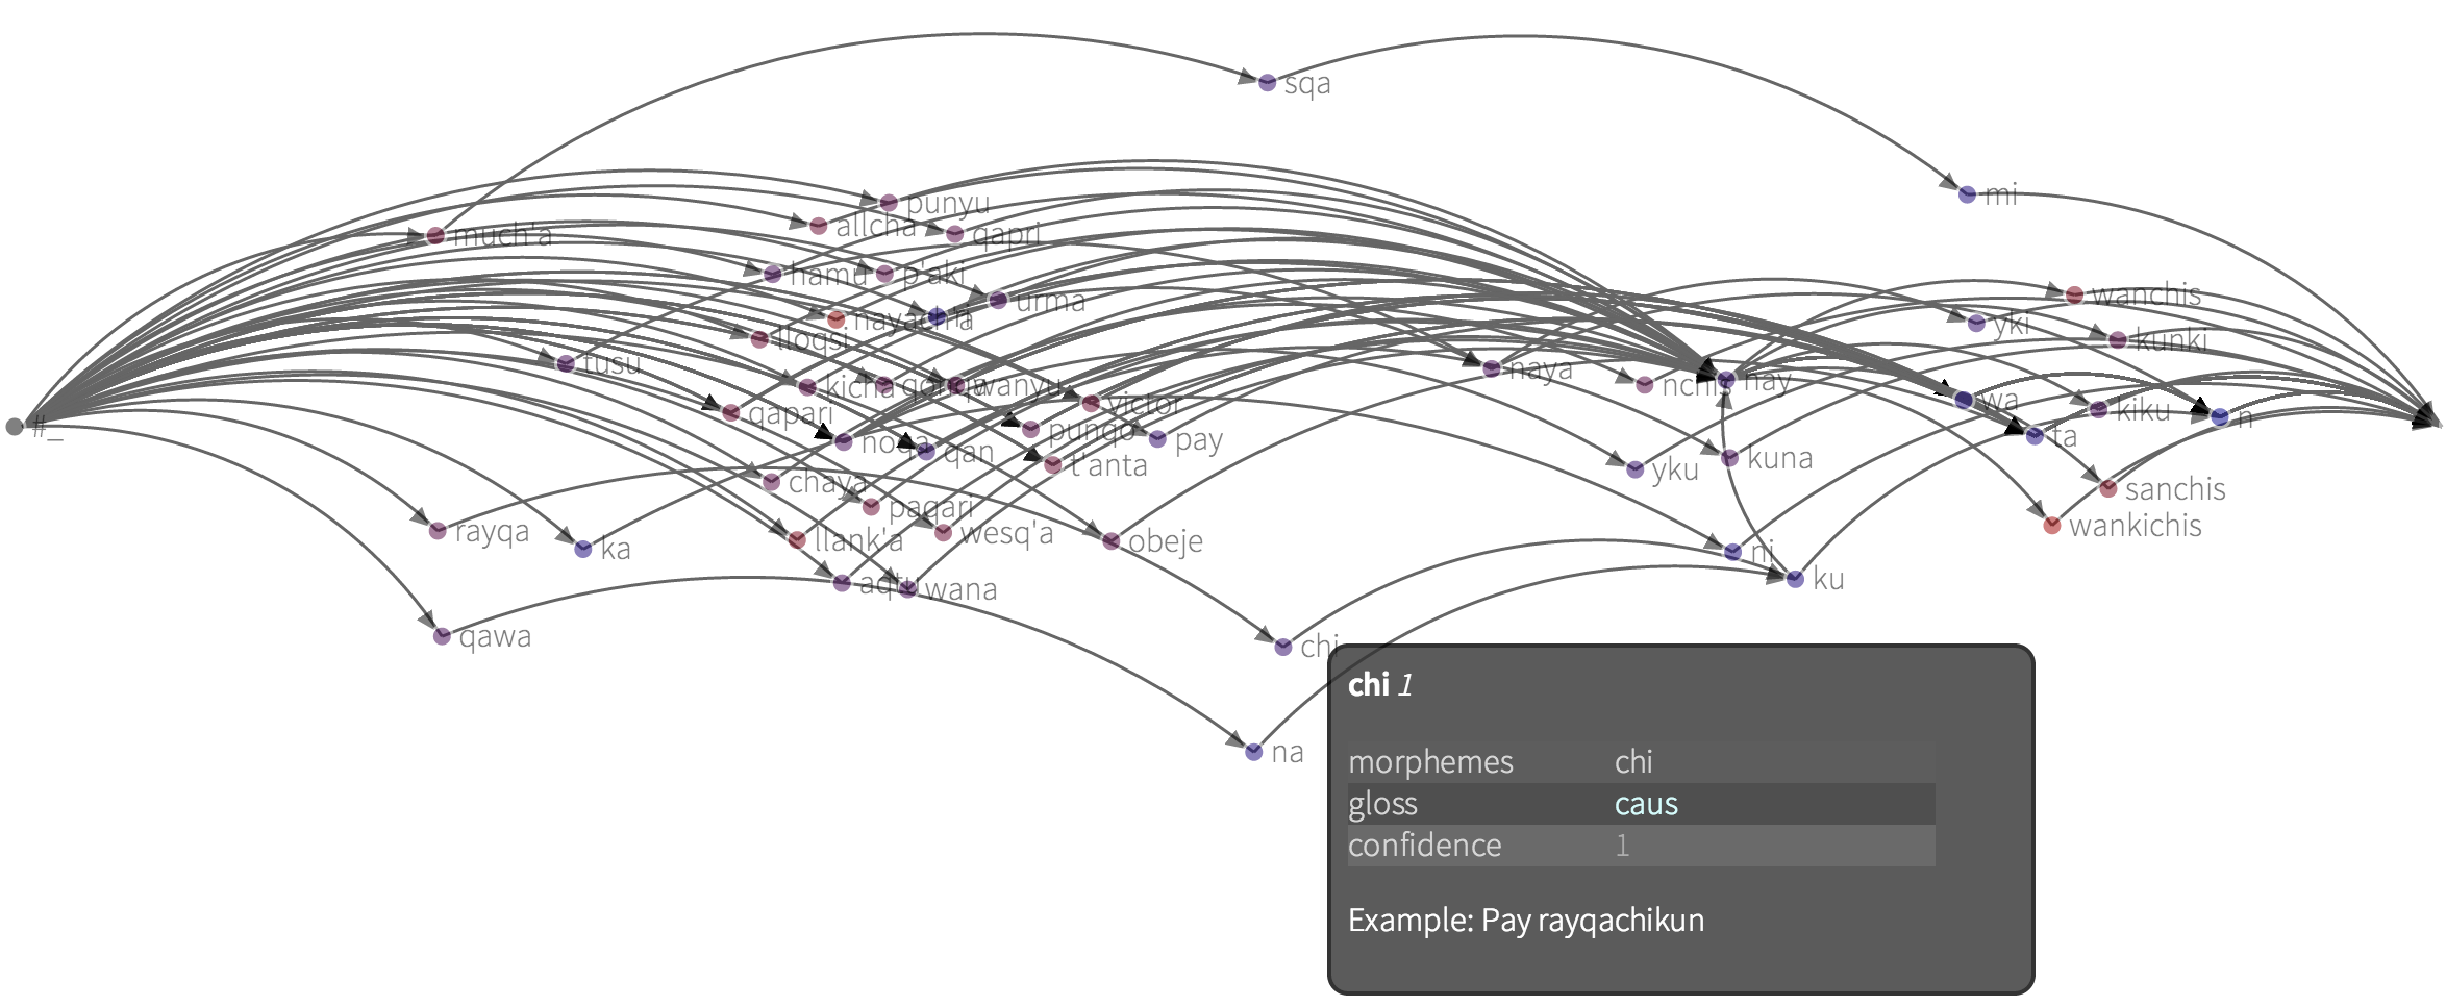
\includegraphics[width=3in]{images/lexicon_browser}
\caption{Screenshot of the Lexicon Browser, a web widget which lets users browse relations between morphemes in their corpus and clean and add declarative knowledge not found in the lexicon training process.}
\label{lexicon_browser_screenshot}
\end{center}
\end{figure}




\subsection{Audio-transcription Alignment}
\label{sec:aligner}

The audio web service is currently capable of performing two services.
\autoref{fig:api-audio}a illustrates the use of the
Prosodylab-Aligner%
\footnote{\url{https://github.com/kylebgorman/Prosodylab-Aligner}} %
tool developed at the McGill Prosody Lab. This service significantly automates
the association of transcriptions to relevant audio clips and therefore helps
to provide a class of data that will prove valuable in applications such as
talking dictionaries and language learning tools. \autoref{fig:api-audio}b
illustrates an additional web service that wraps
FFMPEG%
\footnote{\url{http://www.ffmpeg.org/}} %
and Praat%
\footnote{\url{http://www.praat.org/}} %
to convert any video or audio format to .mp3 and automatically generate
syllable timings and suggested utterance boundaries \cite{DeJong:2009} for automatic chunking of
data.


\begin{figure}[h]
\scriptsize
\begin{verbatim}
a) $ curl --cookie my-cookies.txt\
  --request POST\
  -F files[]=@omi_imitaa.mov\
  -F files[]=@omi_imitaa.lab\
  https://api.lingsync.org/v2/corpora/public-curldemo/
  utterances?process=align

b) $ curl --cookie my-cookies.txt\
  --request POST\
  -F files[]=@omi_imitaa.mov\
  https://api.lingsync.org/v2/corpora/public-curldemo/
  utterances?process=detect
  
c) $ curl --cookie my-cookies.txt\
  --request GET\
  https://api.lingsync.org/v2/corpora/public-curldemo/
  files/omi_imitaa.mp3
 
d) $ curl --cookie my-cookies.txt\
  --request GET\
  https://api.lingsync.org/v2/corpora/public-curldemo/
  files/omi_imitaa.TextGrid
   
\end{verbatim}
\caption{Aligning audio/video and text via Prosodylab-Aligner web service (a) and detecting utterances and syllable timing from audio/video files (b) retrieving web playable audio (c) and TextGrid results (d)}
\normalsize
\label{fig:api-audio}
\end{figure}


\begin{figure}
\begin{center}
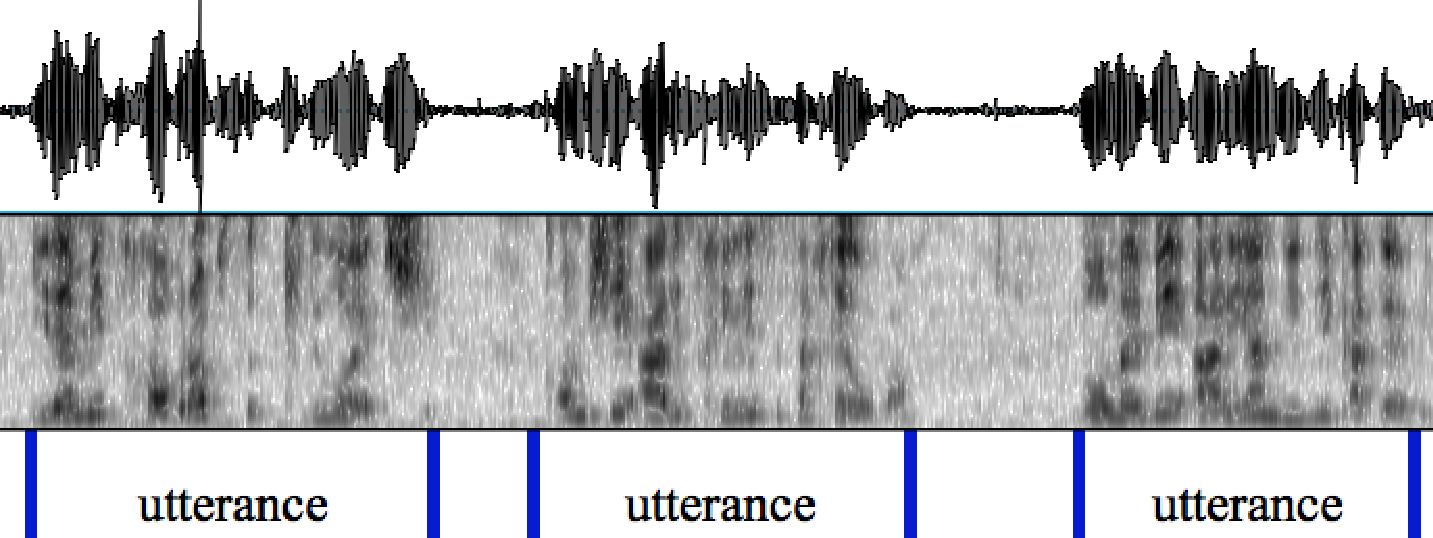
\includegraphics[width=3in]{images/utterance_extraction}
\caption{Screenshot of the utterance extraction results, a web service which converts any audio video into utterance intervals which can be converted into JSON using the PraatTextGridJS library can be converted into datum in LingSync.}
\label{utterance_extraction_screenshot}
\end{center}
\end{figure}


\section{Reusing LingSync/OLD}
\label{open-data}


% BEGIN COMMENT
\begin{comment}
\smalltodo{Examples of actual use
``Show more examples of OLD and LingSync in actual use''
I think that if we remove some of the API stuff (in fitting with other reviewer
comments), we could replace that with more relevant stuff as suggested here. For
example, show what the audio service, the parsers, the search functionality, the
export, the data-sharing, the consistency features, etc. can do and why they are
helpful to fieldworkers broadly construed (i.e., descriptive documentors,
researchers, revitalizers, NLPers).}
\end{comment}
% END COMMENT


LingSync/OLD users are able to make subsets of their data stores publicly
accessible while the language documentation project is active for the advancement of (at least) three distinct endeavors: 1)
theoretical linguistic research, 2) the development of language learning tools for
heritage and second language learners, and 3) the development of data sets for low-resource languages for computational linguistics research. 


%Examples of this last
%endeavor might include the building of better search indexes, classifiers,
%and speech recognition and text-to-speech systems which can then be further
%used to facilitate the use of the data by language communities and researchers.

\subsection{Field linguists}

Field linguists not only enter data but also seek to analyze it. While this may appear to be a trivial claim, it is something which corpus linguistics software overlook. While corpus linguistic tools may be focus on counting occurances or statistics on data coverage, field linguists are looking for fine grained relations between elements in the system which have not yet been documented or understood well enough to be collapsed into typological lists. The Lexicon Browser provides an alternative morpho-syntactic way of browsing a database as opposed to the linear order of text in an elicitation session or text organized by speaker or by tag. Data analysis in LingSync/OLD is facilitated by search  interfaces and the ability to use bots to re-categorize or re-annotate data but in an automatic and suggested-review-execute fashion. Field linguists may also perform cross linguistic searches using MapReduces to normalize data. Primary resources are citable with unique urls and data sets for publication can be annotated stored and discussed in the database itself and directly exported into LaTeX.  Screenshots of these functionalities and many others are provided in \cite{lingsync:2012}.

\textit{Joel: ``suggested-review-execute fashion'' does not make sense to me.}

%	 Lexicon Browser
%	, Data analysis
%	, Cross linguistic search
%	, Citation of primary resources
%	, Publication preparation
%
\subsection{Language Communities}

As discussed in Requirement \autoref{req:inclusive} a majority of LingSync/OLD contributors are doing fieldwork on languages that
are not only under-resourced but also endangered. In this context, the primary
interests of speaker consultants and their communities lie not in theoretical
linguistic research but in the generation of resources that are directly
relevant to the communities' revitalization goals and to increasing the community diaspora's
access to language data. Linguists are now also much more aware of the need to
create records that can be reused by the community and that will still be
available for their descendants \cite[p.129]{Thieberger:2012}, as well as the
importance of designing documentary projects in ways that allow speaker
communities to benefit from the work of an outside researcher \cite{Good:2012}.


\subsubsection{Language Learning}

Descriptive grammars and word lists are of variable utility in the domain of second language acquisition/immersion.
Learning grammars, web-accessible audio (i.e., ``talking'') dictionaries, bilingual dictionaries, monolingual dictionaries, collocation dictionaries, culturally relevant narratives, pedagogical materials, and dedicated language
learning software are generally more valuable to communities, yet these tend to
require a dedicated effort to produce and do not efficiently exploit
opportunities for the reuse of data gathered primarily for research purposes. 
Data gathered for research purposes is often focused on edge cases, usually
using small vocabulary sets to explore less frequent grammatical structures.
In response to this, the Learn X Android app in \autoref{learn_x_screenshot}
was created; it permits language learners to collaboratively create and share
lessons with their peers and mentors. Heritage speakers can benefit from the
same collaborative infrastructure under LingSync/OLD to build a corpus and share
their lessons with each other. 

\begin{figure}
\begin{center}
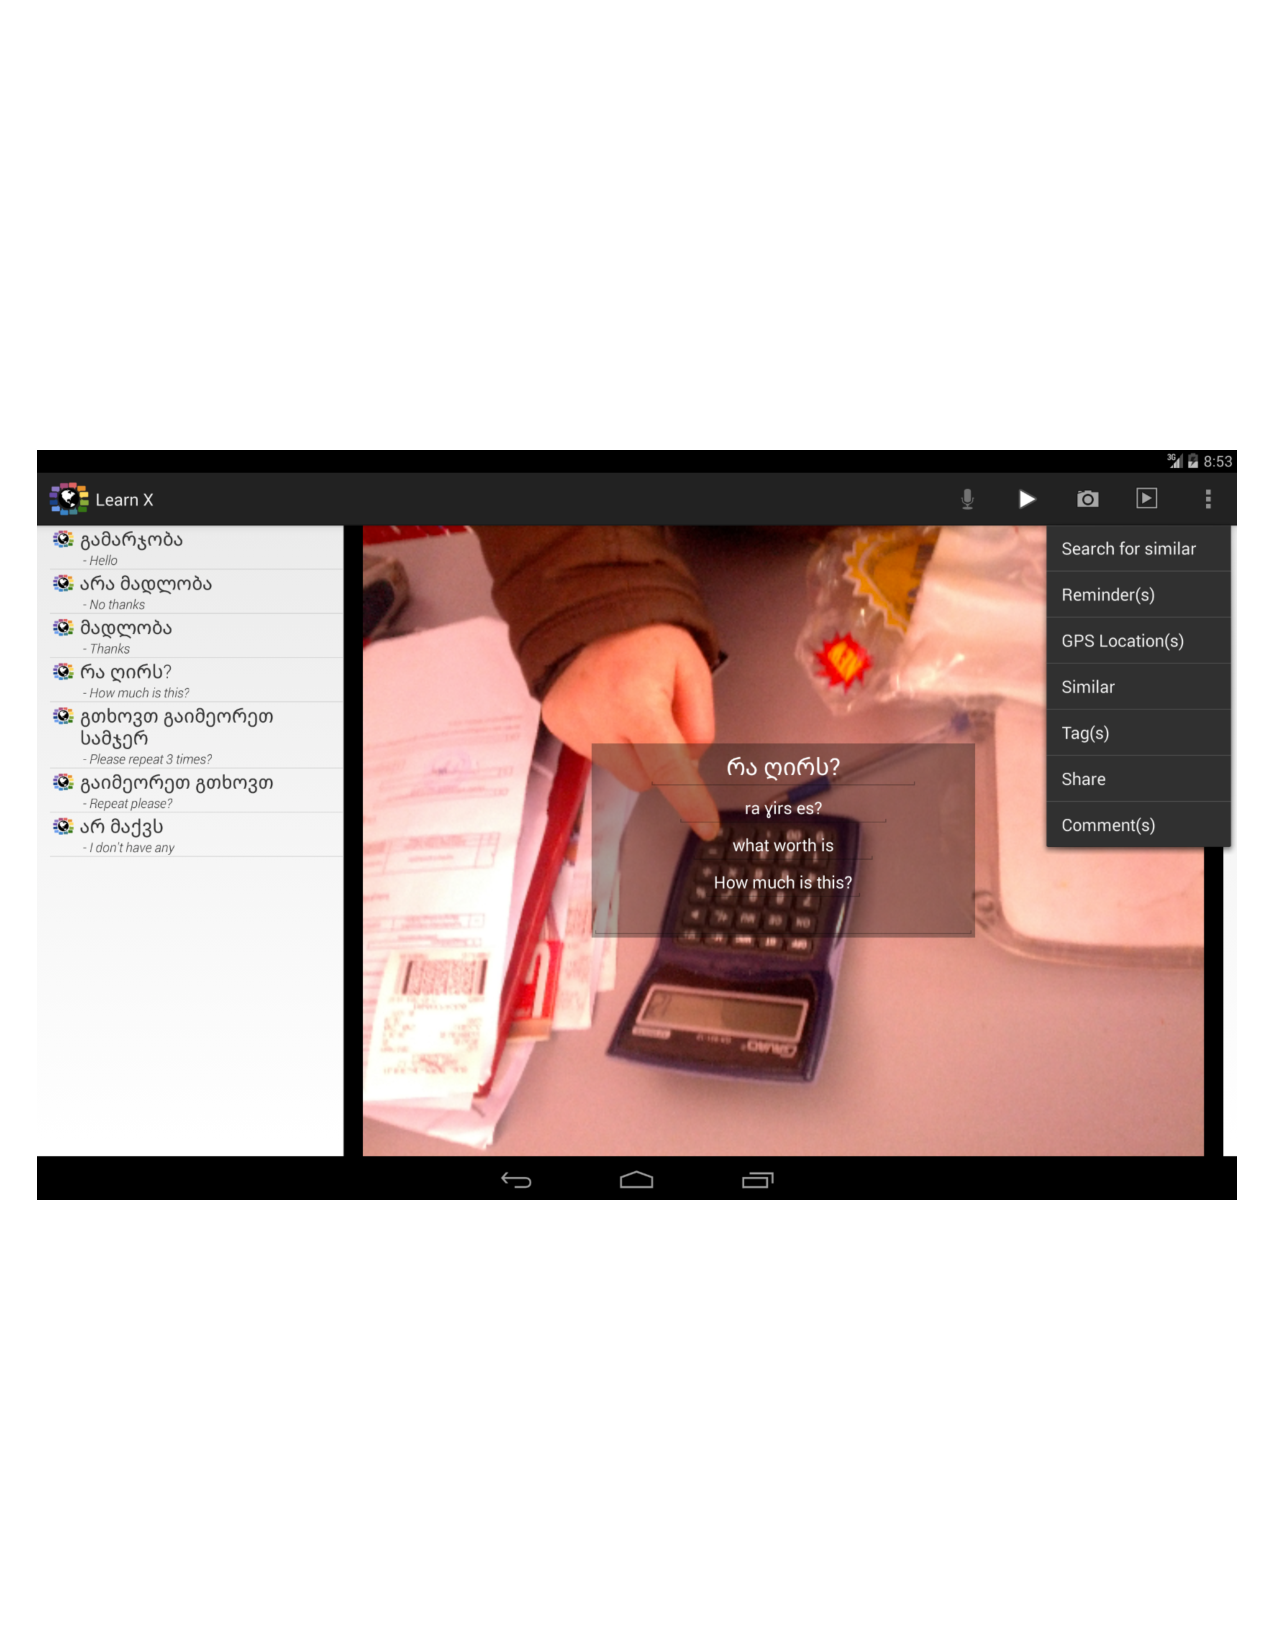
\includegraphics[width=3in]{images/learnX}
\caption{Screenshot of Learn X, an Android app which lets users build language
learning apps using LingSync/OLD.}
\label{learn_x_screenshot}
\end{center}
\end{figure}

LingSync's permissions system was designed so that language community members
and heritage speakers of the language can use the multimedia data collection
features of Android phones (camera, audio, video) to construct their own
language learning lessons which are saved into their own corpus and/or
contributed to a team corpus.

Learn X is freely available for download%
\footnote{\url{https://play.google.com/store/apps/details?id=com.github.opensourcefieldlinguistics.fielddb.lessons.georgian}} %
 as ``Georgian Together" which we are field testing during the Spring 2014 semester with members of the TLG volunteers (Teach Learn Georgia).
Like heritage learners, TLG volunteers spend their time surrounded with the
language, can understand more than they can speak, and what they speak about is
highly dependent on what their family speaks about most. LingSync's
open-endedness and confidentiality settings make it easy for teams to create
and share vocabularies/phrases.
In fact, there are many other contexts which will not be acknowledged or printed
in any online grammar or second language materials, contexts which users can
elect to hide from other users, or share with certain users depending on their
comfort level.

In addition to language learning resources, communities may also benefit from
descriptive grammars, spell checkers, grammar checkers, autocorrect/predictive
typing, subtitling, translation memories, voice writing, content
creation/language representation on the web, and improved access to relevant
web search results. To facilitate access to content, we created a very simple
Georgian transliteration module which makes it so that Georgian speakers can
view text written latin letters by (predominately) iPhone content creators who
do not have access to a Georgian keyboard, also freely available for
download.\footnote{\url{https://chrome.google.com/webstore/detail/kartuli-glasses/ccmledaklimnhjchkcgideafpglhejja}}


\subsection{Computational Linguistics for Low-resource Languages}

Data collected by language documentation projects can also serve the language community indirectly via the construction of computational tools and datasets which can then help software developers build software which enables content in low-resource languages, further facilitating the use of minority languages in digital communication (both spoken and written). Thinking about these data uses before and during data collection with speakers can help field teams think about how to explaining the frequently abstract licensing language to consultants via consent forms as well as potentially concretely identifying the benefits  consultant's participation in the language resources effort has for other members in the community. Language documentation projects can also partner with Software Engineering or Computational Linguistics labs to recompile corpora into gold standard data, and training data, or crowd source annotations, build stemmers, and improve search and information retrieval. Many of these results can be used to build more complex systems including morphological analyzers, machine translation, text to speech systems, speech recognition systems and in some cases such as Georgian even text summarization for local law firms.

During the Spring 2014 semester we are training computer science masters students at the Batumi Shota Rustaveli  State University in how to use CMUSphinx tools to build speech recognition systems which can be delivered to Android smart phone users. Initial pipelines have been prototyped using Bash scripts but will not be in production as an Android app until after the semester is concluded (June 2014). Corpus data are first through a transliteration process to and then used to generate pronunciation dictionaries which serve as input  to the open source Phonetisaurus Libraries \cite{Novak:2012} for the generation of pronunciation entries of novel words. The corpus data is extracted as raw text and used to generate n-gram language models using the open source CMUCLMTK \cite{Clarkson:1997} language model generation scripts which accept a pronunciation dictionary and sentence delimited corpus as input. Acoustic models are adapted from existing acoustic models via the export of utterance lines and corresponding audio and the  \cite{Elmahdy:2010}. Finally, the language specific dictionary, language model, and adapted acoustic model are provided to the PocketSphinx Android library to produce n-best hypothesis for novel audio. While we expect that the result will be poor for most small corpora in the system, automating the model training pipelines can serve to increase interest in the process of speech recognition among software developers from minority language populations  and also encourage language communities to volunteer in the collection and annotation of the sorts of data which are required to have more representative language models and acoustic models \cite{Sarfraz:2010}. 



\subsubsection{API}
%
%
%
%\subsection{Reduce low-level detail}
%
%``Too much space is given to the low-level infrastructure''
%
%I think that this is valid. All of the curl/API examples are useful but maybe not
%appropriate in such a short paper as this. I think we need to focus on the major
%themes.
%
%
%% COMMENTED OUT FOOTNOTE ON "REST"
%%\footnote{REST stands for REpresentational State Transfer
%    %\cite{fielding2000architectural} Here we use the term \textit{RESTful} to
%    %refer to a web site that exposes resources for retrieval and manipulation
%    %in accordance with standard HTTP (Hypertext Transfer Protocol) request
%    %patterns. A RESTful API (application programming interface) essentially
%    %makes it easy to programmatically interact with a web site in predictable
%%ways, thus facilitating its reuse in a variety of contexts.} %
%
%
%
%
%\subsection{Too technical}
%
%\subsubsection{Make the paper more accessible to non-specialists}
%
%``Author needs to make the paper more accessible for a nonspecialist audience.''
%
%
%\subsubsection{Better define terms}
%
%``Define terms (e.g., RESTful).''
%
%I'm planning to use the \LaTeX glossaries package to consistently define all of
%the acronyms and technical jargon. I'm unsure if including an actual glossary
%section in the paper is a good idea though, or if there will even be room for
%this. Unfortunately there aren't many formatting options for the glossary listing
%that is generated. Even making it single-spaced would be an improvement; however,
%the setspace package seems to break the ACL stylesheet \ldots
%
%
%
%\subsection{LingSync}
%
%LingSync exposes a RESTful API where standard combinations of HTTP methods and
%URL patterns correspond to create, read, update, delete, and search operations
%on corpora and \emph{datum} (cf. \autoref{lingsync-auth} and
%\autoref{lingsync-datum}).
%
%
%\begin{figure}[h]
%\scriptsize
%\begin{verbatim}
%$ curl --cookie-jar my-cookies.txt \
%    --header "Content-Type: application/json" \
%    --data '{"name": "public", "password": "none"}' \
%    https://corpus.lingsync.org/_session
%\end{verbatim}
%\normalsize
%\caption{Authenticating to a LingSync corpus service to access publicly
%available corpora.}
%\label{lingsync-auth}
%\end{figure}
%
%\begin{figure}[h]
%\scriptsize
%\begin{verbatim}
%$ curl --request POST --cookie my-cookies.txt \
% --header "Content-Type: application/json" \
% --data '{"collection": "datums", "datumFields": 
% [{"label": "utterance",   "value": "Noqata 
% tusunayawanmi"}, { "label":  "morphemes",
%  "value": "Noqa-ta tusu-naya-wa-n-mi"}]}' 
%  https://corpus.lingsync.org/public-curldemo 
%
%$ curl --cookie my-cookies.txt \
%	https://corpus.lingsync.org/public-curldemo/\
%    _design/pages/_view/datums
%\end{verbatim}
%\normalsize
%\caption{Creating a record and requesting all data.}
%\label{lingsync-datum}
%\end{figure}
%
%
%
%\subsection{OLD}
%
For language documentation teams collaborating with Software Engineering labs
or Computational Linguistics labs LingSync/OLD web services expose a RESTful
\gls{api} for requests on resources.%
\footnote{RESTful means that combinations of \gls{url} patterns and HTTP methods
    names are mapped consistently and transparently to operations on the
    relevant resources. The payloads of all HTTP requests and responses are
\gls{json}}

%Given the consistency and transparency of this API, and given the fact that
%most programming languages have mature libraries for sending and receiving 
%HTTP requests and responses and for serializing to and parsing from JSON, OLD
%resources can easily be re-purposed in a variety of ways.
 \autoref{fig:api-basic}
illustrates the use of the LingSync/OLD \gls{api} for authentication, the creation of an new record, and requesting all records. \autoref{fig:api-search} demonstrates use of the search \gls{api}s. Examples of more sophisticated  \gls{api}s which provide specialized processing for audio/video/image and text  are presented in \autoref{sec:plugins}.

\begin{figure}[h]
\scriptsize

\begin{verbatim}
a) $ curl --cookie-jar my-cookies.txt\
  --request PUT\
  --header "Content-Type: application/json"\
  --data '{"username":"public", "password":"none"}'\
    https://api.lingsync.org/v2/users

b) $ curl --cookie my-cookies.txt\
  --request POST\
  --data '{"transcription": "omi imitaa"}'\
    https://api.lingsync.org/v2/corpora/public-curldemo

c) $ curl --cookie my-cookies.txt\
  --request GET\
    https://api.lingsync.org/v2/corpora/public-curldemo
\end{verbatim}
\caption{\texttt{curl} requests for authentication (a), creating a record (b) and requesting all records (c) }
\normalsize
\label{fig:api-basic}
\end{figure}


%\section{Search}
%\subsection{LingSync}
%
%It is possible to search across all LingSync public corpora using the
%ElasticSearch API. \autoref{lingsync-search} illustrates a search for data
%points which are grammatical and contain \textit{PAST$|$past$|$pst$|$pass} and
%potentially \textit{CAUS$|$CAUSE$|$caus$|$cause} and \textit{ACC$|$Acc$|$acc},
%for users interested in cross-linguistic co-occurrence of accusative and/or
%causative in past contexts.
%
%\begin{figure}[h]
%\scriptsize
%\begin{verbatim}
%$ curl  \
% --data '{"query": {"bool": {"must": [],
% "must_not": [{"term": { "datums.judgement": "*"}}],
% "should": [{"term": {"datums.gloss": "acc" }},{ 
%   "regexp": {"datums.gloss": "cause?"}},{
%   "regexp": {"datums.gloss": "pa?st"}}]}},
% "from": 0, "size": 50, "sort": [], "facets": {}}' \
% http://searchdev.lingsync.org/_search
%\end{verbatim}
%\normalsize
%\caption{Complex cross-corpora search using ElasticSearch's API.}
%\label{lingsync-search}
%\end{figure}
%
%
%
%
%
%It is also possible to search for morphemes in a particular corpus using either
%ElasticSearch, as illustrated in \autoref{lingsync-search}, or CouchDB Map
%Reduce views, as illustrated in \autoref{lingsync-morpheme-search}.
%
%\begin{figure}[h]
%\scriptsize
%\begin{verbatim}
%$ curl  --cookie my-cookies.txt \
%  https://corpus.lingsync.org/lingllama-communitycorpus
%  /_design/demo/_view/datum_by_morpheme
%  ?key="naya"&include_docs=true
%\end{verbatim}
%\normalsize
%\caption{Searching a single corpus using CouchDB's MapReduce API.}
%\label{lingsync-morpheme-search}
%\end{figure}
%
%
%
%\subsection{OLD}
%
%An OLD web service can be searched via a JSON-based interface to the underlying
%RDBMS's query functionality, i.e., an SQL \texttt{WHERE} clause with joins
%handled automatically. \autoref{old-search} illustrates a search that returns
%all \emph{forms} with \textit{cat} as a translation, that are not ungrammatical, whose
%transcriptions begin with \textit{p}, and which have no morpheme gloss
%information. Note the use of the non-standard \texttt{SEARCH} method,%
%\footnote{The \texttt{POST} method with the URL path \texttt{/data/search} is
%a synonym.} %
%the use of nested JSON arrays to represent hierarchically structured filters,
%the implicit join on the translation table, and the use of regular expressions.
%
\begin{figure}[h]
\scriptsize
\begin{verbatim}
a) $ curl --cookie my-cookies.txt\
  --request SEARCH\
  --data '{"query": {"filter": ["and", [
  ["data", "translations", "transcription", "=", "cat"],
  ["or", [["not", ["data", "transcription", "=", "*"]],
          ["data", "grammaticality", "=", null]]],
  ["data", "transcription", "regex", "^p"],
  ["data", "morpheme_gloss", "=", ""]]]}}'\
 https://api.lingsync.org/v2/corpora/public-curldemo
 
b) $ curl --cookie my-cookies.txt\
  --request SEARCH\
  --data '{"query": {"filter":
  ["data", "break_gloss_category", "regex",
    "-wa\|3SG\|Agr( |-|$)"]}}'\
 https://api.lingsync.org/v2/corpora/public-curldemo

c) $ curl --cookie my-cookies.txt\
  --request SEARCH\
  --data '{"tgrep2pattern": "/^[TI]P$/ < (DP << AP)"}'\
  https://api.lingsync.org/v2/corpora
\end{verbatim}
\caption{\texttt{curl} requests for complex search (a), unambiguous morpheme search (b), TGrep2 structural search (c)}
\normalsize
\label{fig:api-search}
\end{figure}
%
%When a morphologically complex \emph{form} is created, an OLD web service generates
%a string representation of the morphological analysis, i.e., morpheme shapes,
%glosses, and categories. This attribute---labeled
%\texttt{break\_gloss\_category}---can be targeted by search filters, thus allowing
%for morphemes to be matched unambiguously. \autoref{old-morpheme-search}
%illustrates how one could search for all \emph{forms} containing a morpheme with the
%shape /wa/, that is glossed \textit{3SG}, and which has category \textit{Agr}.%
%\footnote{The OLD would serialize such a morpheme to \texttt{wa|3SG|Agr}. The
%delimiter used---in this case the vertical line character---can be configured on
%a per-application basis.}
%

%
%An OLD corpus object consisting of a sequence of \emph{form} objects with syntactic
%representations in PTB-compatible bracket notation%
%\footnote{I.e., Penn Treebank bracket notation, cf. \cite{taylor2003penn} and
%\url{http://www.cis.upenn.edu/~treebank/}.} %
%can be written server-side to a treebank file and compiled to a binary format
%that can be searched using the TGrep2 utility. This allows for \emph{forms} to be
%searched according to complex syntactic structural patterns. \autoref{old-tgrep2}
%illustrates a search of corpus 1 for \emph{forms} whose syntactic
%representations have a TP or an IP node that immediately dominates a DP which
%itself dominates an AP, cf.  \cite{rohde2005tgrep2}.
%


\section{Conclusion}


%While the LingSync/OLD project is a yet another endevour in language documenation projects, in this paper we hope to have demonstrated that in the short period since these projects have been active we are already making a significant contribution to reducing fragmentation of efforts.  

In this paper we hoped to have illuminate some of the complexity involved in building language documentation software which has resulted in software fragmentation. We have presented LingSync/OLD,  an open-ended plugin architecture which puts Software Engineering best practices and our collective experience in the language technology industry  to use to solve this fragmentation. The LingSync/OLD project has worked in an itterative fashion, beginning with user interfaces for field linguists in 2012-2013, user interfaces community members and software libraries and training for software developers in 2013-2014, user studies and the dissemination of  potentially novel computational linguistics contributions in 2014-2015 and in the future as the project continues to iterrate.  For technical updates or to collaborate on the project, interested readers may view the project's completed milestones\footnote{\url{https://github.com/OpenSourceFieldlinguistics/FieldDB/issues/milestones?state=closed} }, for user facing updates readers may visit  LingSync.org and OnlineLinguisticDatabase.org. 


\section*{Acknowledgements}

We would like to thank the participants of the Corpus Approaches to Mayan Linguistics Workshop 2012, and the  
Collaborative Language Research Institute 2012  for their feedback and questions, as well as sharing their knowledge and fieldwork experiences. We would also like to thank 
Android Montr\'eal and JavaScript Montr\'eal for their comments and feedback on technical aspects of LingSync presented at meet-ups,
as well as Montreal's start-up community for permitting linguists to immerse themselves in the software culture, 
without which we would not have discovered technologies  used for building social scaleable open ended data management tools.
We would like to express our deep thanks to Tobin Skinner,
Elise McClay,
Louisa Bielig,
MaryEllen Cathcart,
Theresa Deering,
Yuliya Manyakina,
Gretchen McCulloch, 
Hisako Noguchi, 
Brian Doherty, 
Gay Hazan,
Oriana Kilbourn,
Kim Dan Nguyen,
Rakshit Majithiya,
Mietta Lennes,
Nivja de Jong,
Ton Wempe,
Kyle Gorman,
Curtis Mesher,
Beso Beridze, 
Tornike Lasuridze, 
Zviadi Beradze, 
Rezo Turmanidze,
Baata
Jason Smith,
Martin Gausby,
Pablo Duboue,
Xianli Sun as well as countless other linguistics students,  computer science students and open source software developers  who directly or indirectly helped build LingSync/OLD to what it is today and will be in the future. 
We would like to thank the ComputEL workshop reviewers, LingSync/OLD users and would-be users for providing feedback, suggestions,  asking tough questions and sending bug reports, all of which have been instrumental
 in the project's success and helped drive
 the software's development.
 We would like to thank Faryal Abbassi, Farah Abbasi, Tamilla Paghava, Esma Chkhikvadze, Nina Gatenadze, and Mari Mgeladze for their friendship, patience and for sharing their language with us while we share our  technical tools with them.
Finally, we would like to thank Jessica Coon, Alan Bale and Michael
Wagner for their guidance and challenging us to keep the user interfaces simple
and yet flexible, as well as SSHRC Connection Grant (\#611-2012-0001)
and SSHRC Standard Research Grant (\#410-2011-2401) which 
 advocates open-source approaches to knowledge mobilization and
partially funded the students who have doubled as fieldwork research
assistants and interns on the project. All errors and oversights are
naturally our own.  

\printglossary


\bibliographystyle{acl}
\bibliography{bibliography}


\end{document}
